

\begin{figure}[!h]
    \centering
    \resizebox{0.80\textwidth}{!}{
        \begin{tikzpicture}[mindmap,
        level 1 concept/.append style={level distance=130,sibling angle=120},
        ]
        \path[mindmap,concept color=black,text=white]
        node[concept] {Function}
        [clockwise from=0]
        child[concept color=red]{
          node[concept] (exponential) {Exponential Function}
          [clockwise from=30]
          child { node[concept] (range) {Range} }
          child { node[concept] (domain) {Domain} }
        }
        child[concept color=blue] {
            node[concept] (inverse) {Inverse Function}
          [clockwise from=-90]
          child { node[concept] (range) {Range} }
          child { node[concept] (domain) {Domain} }
        }
        child[concept color=green!50!black] {
            node[concept] (logarithm) {Logarithmic Function}
          [clockwise from=150]
          child { node[concept] (range) {Range} }
          child { node[concept] (domain) {Domain} }
        };

        \begin{pgfonlayer}{background}
        \draw [left color=green, right color=red, draw=white,
               decorate,decoration=circle connection bar]
               (exponential) -- (logarithm);
        \draw [left color=blue, right color=red, draw=white,
               decorate,decoration=circle connection bar]
               (exponential) -- (inverse);
        \draw [left color=blue, right color=green!50!black, draw=white,
               decorate,decoration=circle connection bar]
               (logarithm) -- (inverse);
        \end{pgfonlayer}


        \end{tikzpicture}
    }
    \caption{Topics for the second section of the course.}
  \end{figure}



%\include{exponentials/Worksheet-3.1-boring}

\preClass{Coordinate Systems}


\videoLink{Section 3.1}{https://www.youtube.com/playlist?list=PLYHZK3b8UFw2aq4QBoSuTAkPcWN5e-afh}


\begin{enumerate}

\item  Determine if $f(x)=-4x+1$ is one-to-one both algebraically and graphically.
\begin{enumerate}

\item  Graph $f(x)=-4x+1$ and use the graph to determine if $f(x)$ is
  one-to-one.
  \sideNote{Briefly explain your reasoning and do not simply state the name of a theorem or rule.}

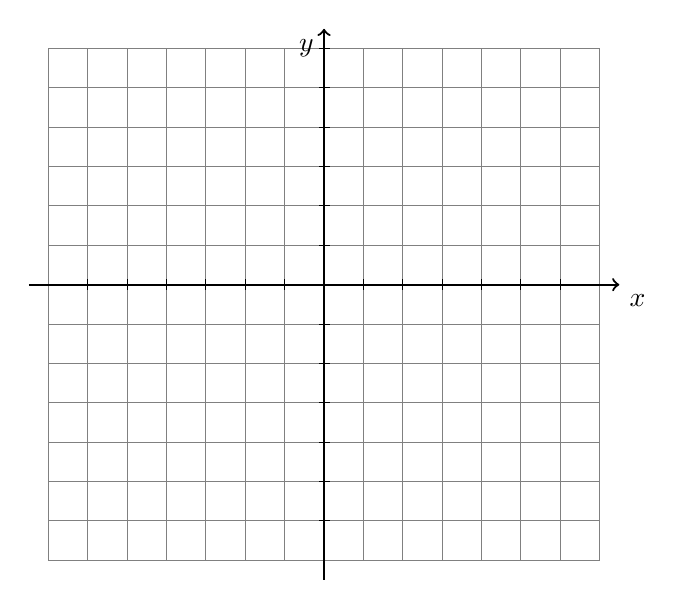
\begin{tikzpicture}[y=.5cm, x=0.5cm,font=\sffamily]
    %% ticks
    \draw[step = 1, gray] (-7,-7) grid (7,6);
    %% axis
    \draw[thick,->] (-7.5,0) -- coordinate (x axis mid) (7.5,0) node[anchor = north west] {$x$};
    \draw[thick,->] (0,-7.5) -- coordinate (y axis mid) (0,6.5) node[anchor = north east] {$y$};
    \foreach \y in {-6,-5,...,-1,1,2,...,6} {
      \draw (2pt, \y) -- (-2pt, \y);
    }
    \foreach \x in {-6,-5,...,-1,1,2,...,6} {
      \draw (\x,2pt) -- (\x,-2pt);
    }

\end{tikzpicture}

\vspace{2em}

\item  Algebraically determine if $f(x)=-4x+1$ is one-to-one.

\vfill


\end{enumerate}



\vfill
\clearpage

\item   Let $f(x)=5x+4$ and $\displaystyle g(x)=\frac{x-4}{5}$.\\
  Use the theorem on inverse functions (function composition) to
  determine whether $f$ and $g$ are inverses.  Show every step.
  
  \vfill


\item Determine the inverse function of $\displaystyle h(x)=\frac{8-x}{3}$.
  
  \vfill




\end{enumerate}





\actTitle{Worksheet 3.1}

\noindent \textbf{Instructions:}  Work together in groups of  3 or 4 to complete the following problems.

Student goals:
\begin{itemize}
\item Determine if a given function is one-to-one. The function can
  be given in graphical, tabular, or algebraic forms.
\item Explicitly show that a function is one-to-one or demonstrate why
  a function is not one-to-one.
\item Determine the inverse of a given function. The function can be
  given in tabular or algebraic forms.
\item Determine the domain and range of the inverse of a function. The
  function can be given in graphical, tabular, or algebraic forms.
\item Limit the domain of a function that is not one-to-one so that an
  inverse can be defined on the resulting restricted domain.
\end{itemize}


For the following set of questions your group should work with three
functions that you will construct. You will start with three basic
functions and transform them into new functions which will be used
throughout the remaining questions.
\begin{enumerate}
\item Use $g(x)=x^2$ and two of the following functions for your
  group.  Along with $g(x)$ choose two from the following functions:
  $$f(x)=x, \quad \quad
  h(x)=x^3, \quad \quad
  j(x)=\frac{1}{x}, \quad \quad
  m(x)=\sqrt{x},  \quad \quad
  p(x)=\sqrt[3]{x}.$$

\item Pick some transformations like shifting, stretching,
  compressing, and reflecting to transform each of your 3
  functions. Give each of your new functions a new name and write your
  3 new functions below.  \sideNote{These are transformations for you
    to choose.}

  \vfill

\item Calculate the domain and range. For each of the 3 new functions.

  \vfill

\clearpage


\item Determine \emph{algebraically} if each of your functions are one-to-one.  

\vfill
\vfill


\item For each of your functions that are not one-to-one, make a
  domain restriction so that the function becomes one-to-one on the
  new domain.

\vfill

\clearpage


\item For each of your functions (including those with new domain restrictions), find their inverse functions.

\vfill

\item Use function composition to verify that the inverse functions you have described are truly inverses to your functions.

\vfill

\clearpage

\item Graph your function and its inverse on the same coordinate axes.  Check that they are properly symmetric to each other.

\begin{multicols}{2}

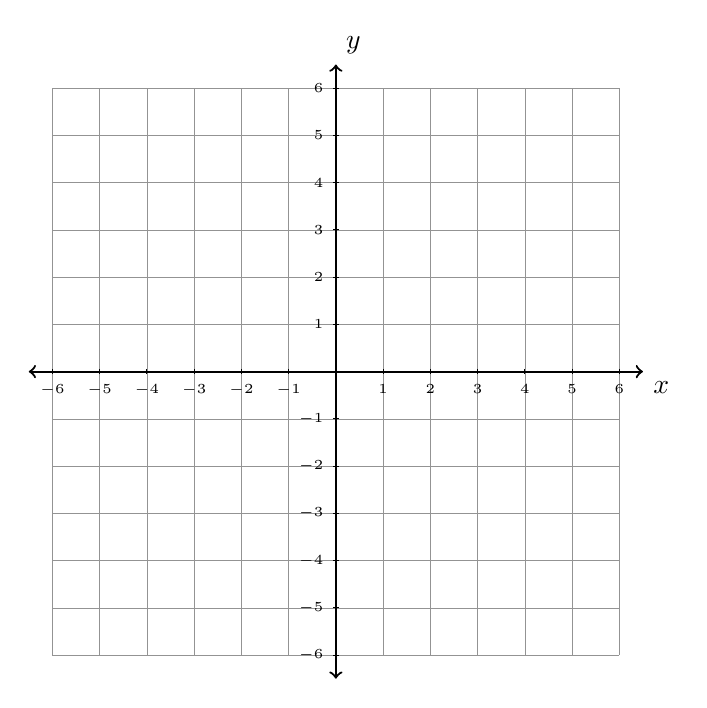
\begin{tikzpicture}[y=.6cm, x=.6cm,font=\sffamily,
	mydot/.style={
    circle,
    fill=white,
    draw,
    outer sep=0pt,
    inner sep=1.5pt
  }]
    %% Add a grid
    \draw[step = 1, gray, very thin,opacity=0.85] (-6, -6) grid (6, 6);
 	%% Draw the axes
	\draw[thick,<->] (-6.5,0) -- coordinate (x axis mid) (6.5,0) node[anchor = north west] {$x$};
    \draw[thick,<->] (0,-6.5) -- coordinate (y axis mid) (0,6.5) node[anchor = south west] {$y$};
    %% Label the y axis
    \foreach \y in {-6,...,-1,1,2,...,6} {
      \draw (1pt, \y) -- (-1pt, \y) node[anchor =  east] {\tiny$\y$};
    }
    %% Label the x axis
    \foreach \x in {-6,...,-1,1,2,...,6} {
      \draw (\x,1pt) -- (\x,-1pt) node[anchor = north] {\tiny$\x$};
    }
    %% Draw the function.
 %   \begin{scope}
 %        \draw[very thick,black] (-3,2) -- (1,1);
 %        \draw[very thick,black] (3.05,1.05) -- (4,3);
    %semi-circle
  %       \draw[very thick, black] (1,1) arc [radius=1, start angle=180, end angle= 5];
     %parabola
     %    \draw[ultra thick, black, domain=-5:0] plot (\x, {(-0.2)*(\x-5)*(\x+5)});
     %dots
     %  \fill[black] (-3, 2) circle[radius=0.5ex];
     %   \fill[black] (1,1) circle[radius=0.5ex];
     %    \fill[black] (4,3) circle[radius=0.5ex];
     %     \draw[very thick, black] (3,1) circle[radius=0.5ex];


   % \end{scope}

    %%\node[above=0.1cm] at (-2,2 )   {\nextXValue};

  \end{tikzpicture}

\vspace{1in}


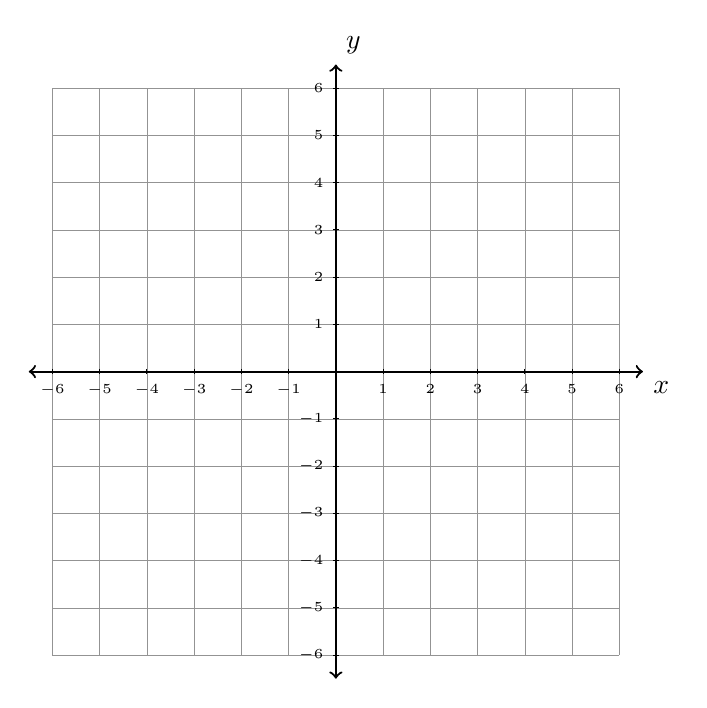
\begin{tikzpicture}[y=.6cm, x=.6cm,font=\sffamily,
	mydot/.style={
    circle,
    fill=white,
    draw,
    outer sep=0pt,
    inner sep=1.5pt
  }]
    %% Add a grid
    \draw[step = 1, gray, very thin,opacity=0.85] (-6, -6) grid (6, 6);
 	%% Draw the axes
	\draw[thick,<->] (-6.5,0) -- coordinate (x axis mid) (6.5,0) node[anchor = north west] {$x$};
    \draw[thick,<->] (0,-6.5) -- coordinate (y axis mid) (0,6.5) node[anchor = south west] {$y$};
    %% Label the y axis
    \foreach \y in {-6,...,-1,1,2,...,6} {
      \draw (1pt, \y) -- (-1pt, \y) node[anchor =  east] {\tiny$\y$};
    }
    %% Label the x axis
    \foreach \x in {-6,...,-1,1,2,...,6} {
      \draw (\x,1pt) -- (\x,-1pt) node[anchor = north] {\tiny$\x$};
    }
    %% Draw the function.
 %   \begin{scope}
 %        \draw[very thick,black] (-3,2) -- (1,1);
 %        \draw[very thick,black] (3.05,1.05) -- (4,3);
    %semi-circle
  %       \draw[very thick, black] (1,1) arc [radius=1, start angle=180, end angle= 5];
     %parabola
     %    \draw[ultra thick, black, domain=-5:0] plot (\x, {(-0.2)*(\x-5)*(\x+5)});
     %dots
     %  \fill[black] (-3, 2) circle[radius=0.5ex];
     %   \fill[black] (1,1) circle[radius=0.5ex];
     %    \fill[black] (4,3) circle[radius=0.5ex];
     %     \draw[very thick, black] (3,1) circle[radius=0.5ex];


   % \end{scope}

    %%\node[above=0.1cm] at (-2,2 )   {\nextXValue};

  \end{tikzpicture}



\columnbreak

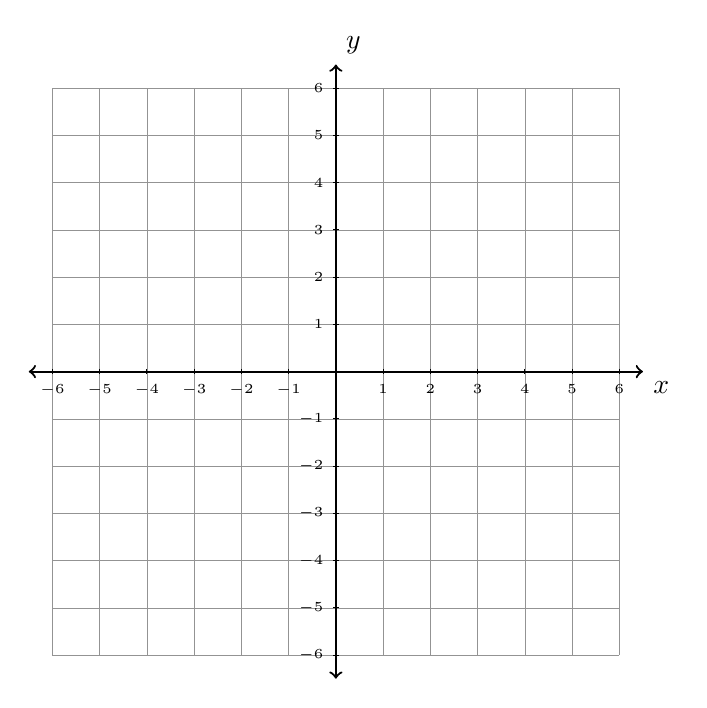
\begin{tikzpicture}[y=.6cm, x=.6cm,font=\sffamily,
	mydot/.style={
    circle,
    fill=white,
    draw,
    outer sep=0pt,
    inner sep=1.5pt
  }]
    %% Add a grid
    \draw[step = 1, gray, very thin,opacity=0.85] (-6, -6) grid (6, 6);
 	%% Draw the axes
	\draw[thick,<->] (-6.5,0) -- coordinate (x axis mid) (6.5,0) node[anchor = north west] {$x$};
    \draw[thick,<->] (0,-6.5) -- coordinate (y axis mid) (0,6.5) node[anchor = south west] {$y$};
    %% Label the y axis
    \foreach \y in {-6,...,-1,1,2,...,6} {
      \draw (1pt, \y) -- (-1pt, \y) node[anchor =  east] {\tiny$\y$};
    }
    %% Label the x axis
    \foreach \x in {-6,...,-1,1,2,...,6} {
      \draw (\x,1pt) -- (\x,-1pt) node[anchor = north] {\tiny$\x$};
    }
    %% Draw the function.
 %   \begin{scope}
 %        \draw[very thick,black] (-3,2) -- (1,1);
 %        \draw[very thick,black] (3.05,1.05) -- (4,3);
    %semi-circle
  %       \draw[very thick, black] (1,1) arc [radius=1, start angle=180, end angle= 5];
     %parabola
     %    \draw[ultra thick, black, domain=-5:0] plot (\x, {(-0.2)*(\x-5)*(\x+5)});
     %dots
     %  \fill[black] (-3, 2) circle[radius=0.5ex];
     %   \fill[black] (1,1) circle[radius=0.5ex];
     %    \fill[black] (4,3) circle[radius=0.5ex];
     %     \draw[very thick, black] (3,1) circle[radius=0.5ex];


   % \end{scope}

    %%\node[above=0.1cm] at (-2,2 )   {\nextXValue};

  \end{tikzpicture}
  

\vspace{1in}


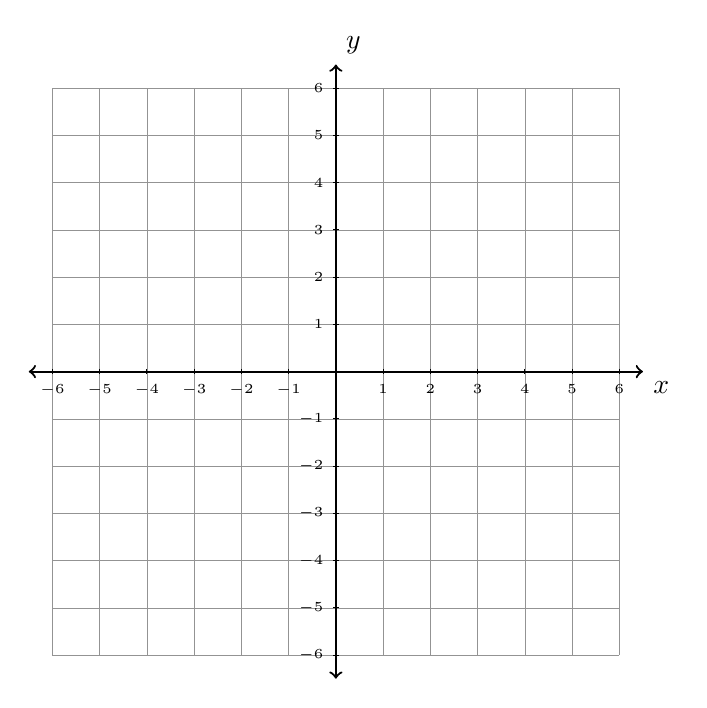
\begin{tikzpicture}[y=.6cm, x=.6cm,font=\sffamily,
	mydot/.style={
    circle,
    fill=white,
    draw,
    outer sep=0pt,
    inner sep=1.5pt
  }]
    %% Add a grid
    \draw[step = 1, gray, very thin,opacity=0.85] (-6, -6) grid (6, 6);
 	%% Draw the axes
	\draw[thick,<->] (-6.5,0) -- coordinate (x axis mid) (6.5,0) node[anchor = north west] {$x$};
    \draw[thick,<->] (0,-6.5) -- coordinate (y axis mid) (0,6.5) node[anchor = south west] {$y$};
    %% Label the y axis
    \foreach \y in {-6,...,-1,1,2,...,6} {
      \draw (1pt, \y) -- (-1pt, \y) node[anchor =  east] {\tiny$\y$};
    }
    %% Label the x axis
    \foreach \x in {-6,...,-1,1,2,...,6} {
      \draw (\x,1pt) -- (\x,-1pt) node[anchor = north] {\tiny$\x$};
    }
    %% Draw the function.
 %   \begin{scope}
 %        \draw[very thick,black] (-3,2) -- (1,1);
 %        \draw[very thick,black] (3.05,1.05) -- (4,3);
    %semi-circle
  %       \draw[very thick, black] (1,1) arc [radius=1, start angle=180, end angle= 5];
     %parabola
     %    \draw[ultra thick, black, domain=-5:0] plot (\x, {(-0.2)*(\x-5)*(\x+5)});
     %dots
     %  \fill[black] (-3, 2) circle[radius=0.5ex];
     %   \fill[black] (1,1) circle[radius=0.5ex];
     %    \fill[black] (4,3) circle[radius=0.5ex];
     %     \draw[very thick, black] (3,1) circle[radius=0.5ex];


   % \end{scope}

    %%\node[above=0.1cm] at (-2,2 )   {\nextXValue};

  \end{tikzpicture}
  
  
\end{multicols}

\clearpage

\item Determine whether or not each relationship below is a function.
  For each relationship that is a function briefly discuss whether or
  not it is a one-to-one function. Briefly explain your reasoning. if
  a function is not one-to-one determine a restriction on the domain
  so that it is one-to-one on the restricted domain.

  \begin{enumerate}
  \item ~ \\
  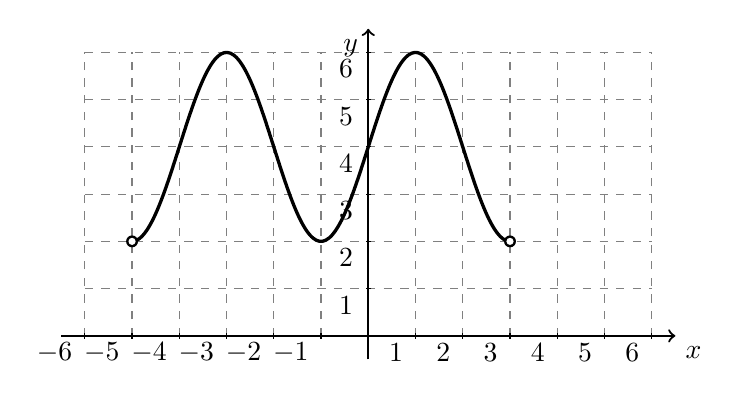
\begin{tikzpicture}[y=0.6cm, x=0.6cm,font=\sffamily]
    %% ticks
    \draw[step = 1, gray,dashed] (-6,0) grid (6,6);
    %% axis
    \draw[thick,->] (-6.5,0) -- coordinate (x axis mid) (6.5,0) node[anchor = north west] {$x$};
    \draw[thick,->] (0,-.5) -- coordinate (y axis mid) (0,6.5) node[anchor = north east] {$y$};
    \foreach \y in {1,2,...,6} {
      \draw (1pt, \y) -- (-1pt, \y) node[yshift=-6,xshift=-1,anchor=east] {$\y$};
    }
    \foreach \x in {-6,-5,...,-1,1,2,...,6} {
      \draw (\x,1pt) -- (\x,-1pt) node[yshift=-5,xshift=-1,anchor=east] {$\x$};
    }

    \begin{scope}
      %\clip(-4,-1) rectangle (8,5);
      \draw[scale=1.0,domain=-4:4,smooth,variable=\x,very thick,black,samples=120] 
           plot ({\x-1},{4+2*sin(deg(pi*\x/2-pi/2))});
      \fill[black] (-5,2) circle [radius=0.5ex];
      \fill[white] (-5,2) circle [radius=0.3ex];
      \fill[black] ( 3,2) circle [radius=0.5ex];
      \fill[white] ( 3,2) circle [radius=0.3ex];
    \end{scope}

  \end{tikzpicture}

  \vfill
  
  \item ~ \\
    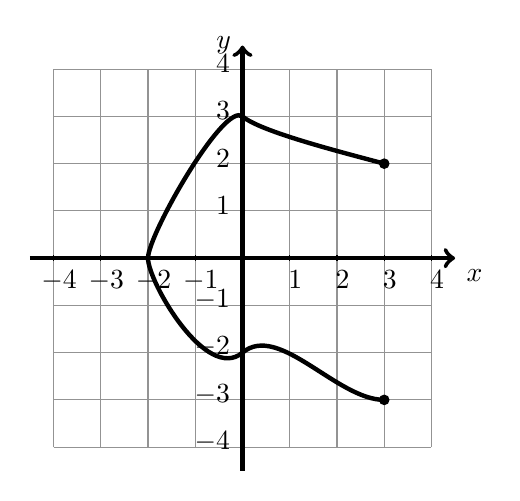
\begin{tikzpicture}[y=0.6cm, x=0.6cm,font=\sffamily]
      \draw[step = 1, gray, thin,opacity=0.85] (-4,-4) grid (4,4);
      \draw[black,ultra thick,->] (-4.5,0) -- (4.5,0) node[anchor=north west] {$x$};
      \draw[black,ultra thick,->] (0,-4.5) -- (0,4.5) node[anchor=east] {$y$};
      \foreach \y in {-4,-3,-2,-1,1,2,3,4} {
        \draw (1pt, \y) -- (-1pt, \y) node[anchor = east,yshift=2] {$\y$};
        \draw (\y,1pt) -- (\y,-1pt) node[anchor = north,xshift=2] {$\y$};
      }
      \draw[ultra thick,black] (3, -3) .. controls +(0:-1) and +(40:1) .. (0, -2)
                    ( 0,-2) .. controls +( 40:-1.0) and +(90:-0.5) .. (-2, 0)
                    (-2, 0) .. controls +( 90:0.5) and +(-40:-0.5) .. (0,3)
                    ( 0, 3) .. controls +(-40:0.5) and +(-15:-1) .. (3, 2);
          \draw[black,fill=black]  (3,-3) circle (0.1);
          \draw[black,fill=black]  (3, 2) circle (0.1);

    \end{tikzpicture}

    \vfill
    
    \item ~ \\
    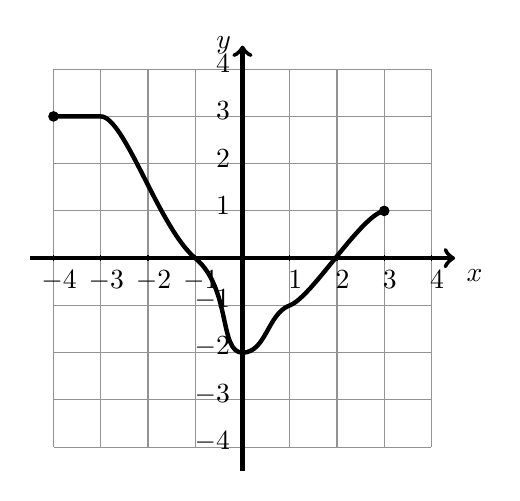
\begin{tikzpicture}[y=0.6cm, x=0.6cm,font=\sffamily]
      \draw[step = 1, gray, thin,opacity=0.85] (-4,-4) grid (4,4);
      \draw[black,ultra thick,->] (-4.5,0) -- (4.5,0) node[anchor=north west] {$x$};
      \draw[black,ultra thick,->] (0,-4.5) -- (0,4.5) node[anchor=east] {$y$};
      \foreach \y in {-4,-3,-2,-1,1,2,3,4} {
        \draw (1pt, \y) -- (-1pt, \y) node[anchor = east,yshift=2] {$\y$};
        \draw (\y,1pt) -- (\y,-1pt) node[anchor = north,xshift=2] {$\y$};
      }
      \draw[ultra thick,black]
                    (-4,3)  .. controls +(0:1) and +(180:0.5) .. (-3,3)
                    (-3, 3) .. controls +(0:0.5) and +(140:1) .. (-1, 0)
                    ( -1,0) .. controls +( 140:-1) and +(180:0.5) .. (0, -2)
                    ( 0, -2) .. controls +(0:0.5) and +(200:0.5) .. (1,-1)
                    ( 1, -1) .. controls +(200:-0.5) and  +(190:0.5) .. (3,1);
          \draw[black,fill=black]  (-4,3) circle (0.1);
          \draw[black,fill=black]  (3, 1) circle (0.1);

    \end{tikzpicture}

    \vfill
    
  \end{enumerate}

\end{enumerate}

\hwTitle{Section 3.1}

\begin{enumerate}
\item The graph of a function, $h$, is given in the plot below, and a
  table is given for all of the values of a function, $g$. Use the
  information in the graph and the table to answer each of the
  questions below. \textbf{If a value does not exist briefly explain
    why.}

  \begin{tabular}{p{0.7\textwidth}p{0.2\textwidth}}
    \begin{minipage}{0.7\linewidth}
      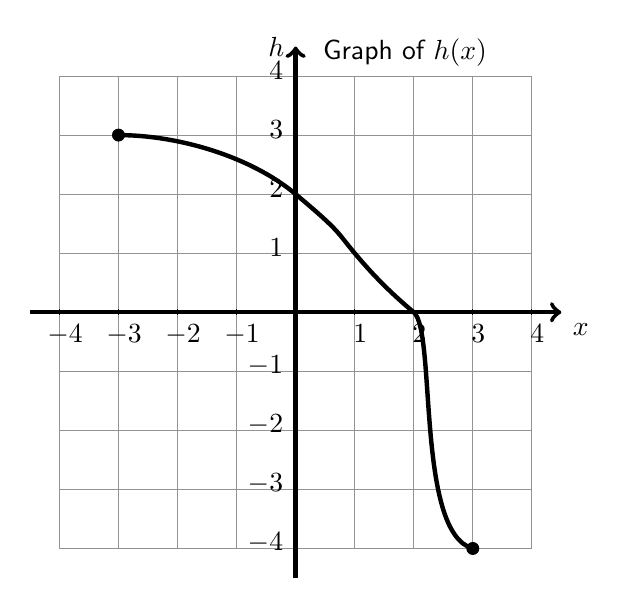
\begin{tikzpicture}[y=0.75cm, x=0.75cm,font=\sffamily]
        \draw[step = 1, gray, thin,opacity=0.85] (-4,-4) grid (4,4);
        \draw[black,ultra thick,->] (-4.5,0) -- (4.5,0) node[anchor=north west] {$x$};
        \draw[black,ultra thick,->] (0,-4.5) -- (0,4.5) node[anchor=east] {$h$};
        \node[black,anchor=south west] at (0.3,4) {Graph of $h(x)$};
        \foreach \y in {-4,-3,-2,-1,1,2,3,4} {
          \draw (1pt, \y) -- (-1pt, \y) node[anchor = east,yshift=2] {$\y$};
          \draw (\y,1pt) -- (\y,-1pt) node[anchor = north,xshift=2] {$\y$};
        }
        %% Draw the function.
        \begin{scope}
          \draw[ultra thick,black] (-3, 3) .. controls +(0:1) and +(-40:-1) .. (0, 2)
                    ( 0, 2) .. controls +(-40:1.0) and +(-50:-0.5) .. (1, 1)
                    ( 1, 1) .. controls +(-50:0.5) and +(-40:-0.5) .. (2,0)
                    ( 2,0) .. controls +(-40:0.5) and +(-15:-1) .. (3, -4);
          \draw[black,fill=black]  (-3,3) circle (0.1);
          \draw[black,fill=black]  (3,-4) circle (0.1);
        \end{scope}
      \end{tikzpicture}
    \end{minipage}
    &
      \begin{minipage}{0.2\linewidth}
        \begin{tabular}{r|r}
          $x$ & $g(x)$ \\ \hline
          0 & 5 \\
          1 & 0 \\
          2 & -3 \\
          3 & 1 \\
          4 & 3 
        \end{tabular}
      \end{minipage}
  \end{tabular}

  \begin{enumerate}
  \item  Is the function $h$ 1-1? (Briefly justify your answer.)
  \item  Determine the value of $g(h(2))$.
  \item  Determine the value of  $h(g(2))$.
  \item  Determine the value of $g^{-1}(h(3))$.
  \item  Determine the value of $g(h^{-1}(3))$.
  \item  Determine the range and domain of $g^{-1}$.
  \item  Determine the range and domain of $h^{-1}$.
  \end{enumerate}

\item The following questions refer to the functions whose graphs are
  given below.x

    \begin{tabular}{p{0.5\textwidth}p{0.5\textwidth}}
    \begin{minipage}{0.5\linewidth}
      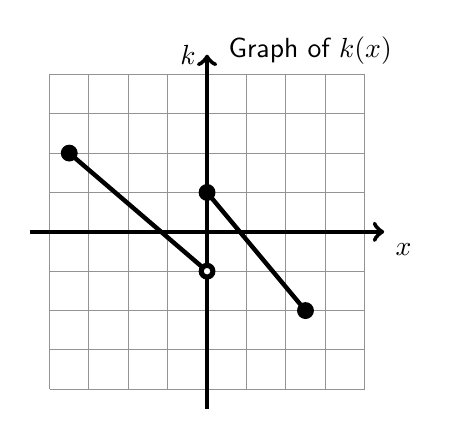
\begin{tikzpicture}[y=0.5cm, x=0.5cm,font=\sffamily]
        \draw[step = 1, gray, thin,opacity=0.85] (-4,-4) grid (4,4);
        \draw[black,ultra thick,->] (-4.5,0) -- (4.5,0) node[anchor=north west] {$x$};
        \draw[black,ultra thick,->] (0,-4.5) -- (0,4.5) node[anchor=east] {$k$};
        \node[black,anchor=south west] at (0.3,4) {Graph of $k(x)$};
        %\foreach \y in {-4,-3,-2,-1,1,2,3,4} {
        %  \draw (1pt, \y) -- (-1pt, \y) node[anchor = east,yshift=2] {$\y$};
        %  \draw (\y,1pt) -- (\y,-1pt) node[anchor = north,xshift=2] {$\y$};
        %}
        %% Draw the function.
        \begin{scope}
          \draw[black,ultra thick] (-3.5,2) -- (0,-1);
          \draw[black,ultra thick] (0,1)    -- (2.5,-2);
          \draw[black,fill=black]  (-3.5,2) circle (0.2);
          \draw[black,fill=black]  (0,-1) circle (0.2);
          \draw[black,fill=white]  (0,-1) circle (0.1);
          \draw[black,fill=black]  (0, 1) circle (0.2);
          \draw[black,fill=black]  (2.5,-2) circle (0.2);
        \end{scope}
      \end{tikzpicture}
    \end{minipage}
    &
      \begin{minipage}{0.5\linewidth}
      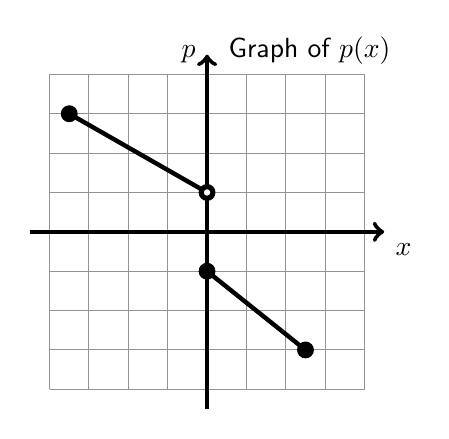
\begin{tikzpicture}[y=0.5cm, x=0.5cm,font=\sffamily]
        \draw[step = 1, gray, thin,opacity=0.85] (-4,-4) grid (4,4);
        \draw[black,ultra thick,->] (-4.5,0) -- (4.5,0) node[anchor=north west] {$x$};
        \draw[black,ultra thick,->] (0,-4.5) -- (0,4.5) node[anchor=east] {$p$};
        \node[black,anchor=south west] at (0.3,4) {Graph of $p(x)$};
        %\foreach \y in {-4,-3,-2,-1,1,2,3,4} {
        %  \draw (1pt, \y) -- (-1pt, \y) node[anchor = east,yshift=2] {$\y$};
        %  \draw (\y,1pt) -- (\y,-1pt) node[anchor = north,xshift=2] {$\y$};
        %}
        %% Draw the function.
        \begin{scope}
          \draw[black,ultra thick] (-3.5,3) -- (0,1);
          \draw[black,ultra thick] (0,-1)    -- (2.5,-3);
          \draw[black,fill=black]  (-3.5,3) circle (0.2);
          \draw[black,fill=black]  (0,1) circle (0.2);
          \draw[black,fill=white]  (0,1) circle (0.1);
          \draw[black,fill=black]  (0,-1) circle (0.2);
          \draw[black,fill=black]  (2.5,-3) circle (0.2);
        \end{scope}
      \end{tikzpicture}
      \end{minipage}
    \end{tabular}

    \begin{enumerate}
    \item Determine the domain of $k(x)$ and determine the set of
      values of $x$ over which the function is decreasing. Is the
      function, $k(x)$, one-to-one? (Briefly justify your reasoning.)
    \item Determine the domain of $p(x)$ and determine the set of
      values of $x$ over which the function is decreasing. Is the
      function, $p(x)$, one-to-one? (Briefly justify your reasoning.)
    \item Are $k(x)$ and $p(x)$ strictly decreasing functions? If a
      function is strictly decreasing is the function one-to-one?
      (Briefly justify your reasoning.)
    \end{enumerate}

  \item The graph of a function is given below. Determine whether or
    not an inverse for the function exists. If not determine a
    restriction on the domain so that the function is invertable on
    your restricted domain. Your restricted domain should allow you to
    invert the function for any value of $y$ in the range of the
    original function.

      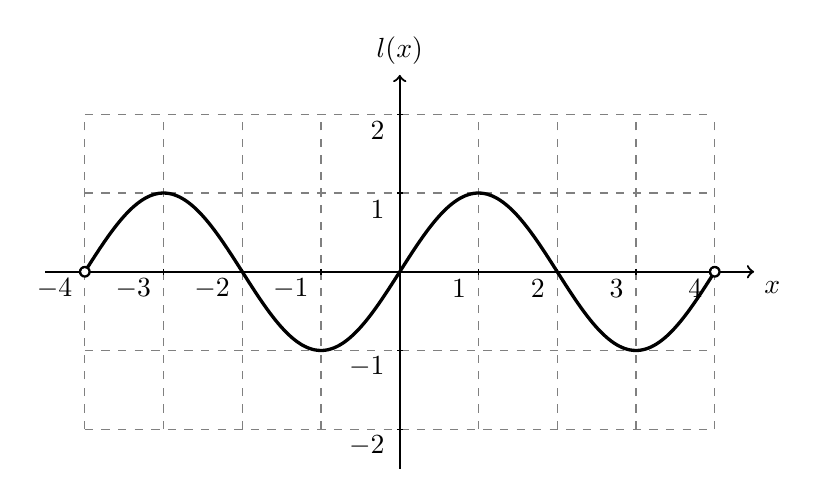
\begin{tikzpicture}[y=1.0cm, x=1.0cm,font=\sffamily]
    %% ticks
    \draw[step = 1, gray,dashed] (-4,-2) grid (4,2);
    %% axis
    \draw[thick,->] (-4.5,0) -- coordinate (x axis mid) (4.5,0) node[anchor = north west] {$x$};
    \draw[thick,->] (0,-2.5) -- coordinate (y axis mid) (0,2.5) node[anchor = south] {$l(x)$};
    \foreach \y in {-2,-1,1,2} {
      \draw (1pt, \y) -- (-1pt, \y) node[yshift=-6,xshift=-1,anchor=east] {$\y$};
    }
    \foreach \x in {-4,-3,...,-1,1,2,...,4} {
      \draw (\x,1pt) -- (\x,-1pt) node[yshift=-5,xshift=-1,anchor=east] {$\x$};
    }

    \begin{scope}
      %\clip(-4,-1) rectangle (8,5);
      \draw[scale=1.0,domain=-4:4,smooth,variable=\x,very thick,black,samples=120] 
           plot ({\x},{sin(deg(pi*\x/2))});
      \fill[black] (-4,0) circle [radius=0.5ex];
      \fill[white] (-4,0) circle [radius=0.3ex];
      \fill[black] ( 4,0) circle [radius=0.5ex];
      \fill[white] ( 4,0) circle [radius=0.3ex];
    \end{scope}

  \end{tikzpicture}

\item The equation for a function, $j(x)$, is given below, and a table
  is given for all of the values of a function, $v(x)$. Use the
  formula and the table to answer each of the questions
  below. \textbf{If a value does not exist briefly explain why.}

  \begin{tabular}{p{0.3\textwidth}p{0.3\textwidth}}
    \begin{minipage}{0.3\linewidth}
      \begin{eqnarray*}
        j(x) & = & |x|,
      \end{eqnarray*}
    \end{minipage}
    &
      \begin{minipage}{0.3\linewidth}
        \begin{tabular}{r|r}
          $x$ & $v(x)$ \\ \hline
          0 & 10 \\
          1 &  8 \\
          2 &  4 \\
          3 &  0 \\
          4 & -2
        \end{tabular}
      \end{minipage}
  \end{tabular}

  \begin{enumerate}
  \item  Is the function $j$ 1-1? (Briefly justify your answer.)
  \item  Is the function $v$ 1-1? (Briefly justify your answer.)
  \item  Determine the value of $j(v(2))$.
  \item  Determine the value of  $v(j(-2))$.
  \item  Determine the value of $v^{-1}(j(-3))$.
  \item  Determine the value of $v(j^{-1}(-3))$.
  \item  Determine the range and domain of $v^{-1}$.
  \end{enumerate}


\end{enumerate}




\preClass{Coordinate Systems}


\videoLink{Section 3.2}{https://www.youtube.com/playlist?list=PLYHZK3b8UFw3OE2GrAT4IExxBw5meagdH}


\begin{enumerate}

\item  Graph the following functions.
\begin{enumerate}

\item  Graph $\displaystyle f(x)=\left(\frac{1}{4}\right)^x$ along with it's asymptote.  (It is helpful to plot values for $x=0, 1, -1$.)\\
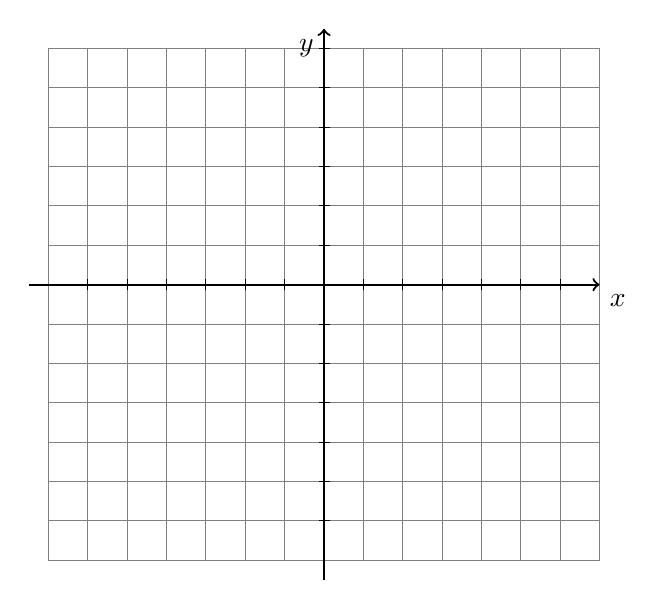
\begin{tikzpicture}[y=.5cm, x=0.5cm,font=\sffamily]
    %% ticks
    \draw[step = 1, gray] (-7,-7) grid (7,6);
    %% axis
    \draw[thick,->] (-7.5,0) -- coordinate (x axis mid) (7,0) node[anchor = north west] {$x$};
    \draw[thick,->] (0,-7.5) -- coordinate (y axis mid) (0,6.5) node[anchor = north east] {$y$};
    \foreach \y in {-6,-5,...,-1,1,2,...,6} {
      \draw (2pt, \y) -- (-2pt, \y);
    }
    \foreach \x in {-6,-5,...,-1,1,2,...,6} {
      \draw (\x,2pt) -- (\x,-2pt);
    }

\end{tikzpicture}



\item  Transform part $(a)$ to graph $\displaystyle g(x)=\left(\frac{1}{4}\right)^{x+3}-2$ along with it's asymptote.\\

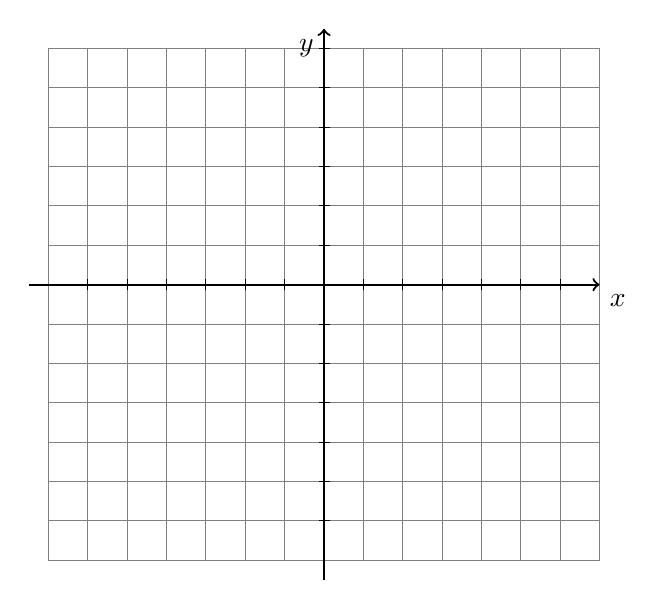
\begin{tikzpicture}[y=.5cm, x=0.5cm,font=\sffamily]
    %% ticks
    \draw[step = 1, gray] (-7,-7) grid (7,6);
    %% axis
    \draw[thick,->] (-7.5,0) -- coordinate (x axis mid) (7,0) node[anchor = north west] {$x$};
    \draw[thick,->] (0,-7.5) -- coordinate (y axis mid) (0,6.5) node[anchor = north east] {$y$};
    \foreach \y in {-6,-5,...,-1,1,2,...,6} {
      \draw (2pt, \y) -- (-2pt, \y);
    }
    \foreach \x in {-6,-5,...,-1,1,2,...,6} {
      \draw (\x,2pt) -- (\x,-2pt);
    }

\end{tikzpicture}


\vfill


\end{enumerate}



\vfill
\newpage

\item  Suppose that \$5000 is invested and pays 6.5\% per year under the following compounding options.  Determine the total amount in the account after 10 years with each option.

\begin{enumerate}
\item  Compounded monthly
\vfill
\item  Compounded continuously
\vfill

\end{enumerate}




\end{enumerate}






\actTitle{Worksheet 3.2}

\noindent \textbf{Instructions:}  Work together in groups of  3 or 4 to complete the following problems.

Student goals:
\begin{itemize}
  \item Use the definition of an exponential function to define a
    function describing a situation given in written, verbal, or
    graphical form.
  \item Use the properties and operations of exponential functions to
    solve for any variable in an expression that has exponential functions.
  \item Be able to graph exponential functions. Be able to compare and
    identify different exponential functions whose parameters differ.
  \item Given the parameters associated with multiple exponential
    grow/decay equations determine the general behaviour and compare
    the relative growth or decay of the different equations.
  \item Determine the equation for the balance of a bank account or
    credit debt for compound interest given a written description of
    the situation.
  \item Determine the equation for the value of an exponential
    growth/decay problem given a written description of the
    situation. Be able to identify if a situation results in either
    growth or decay.
\end{itemize}



\subsection{Exponential Functions}
\begin{enumerate}
\item Which of the following equations represent exponential
  functions?
  {Circle the exponential functions.}
  $$f(x)=2x+1, \quad
  g(x)=-4^x, \quad
  h(x)=1^x, \quad
  j(x)=3(2)^x,  \quad
  m(x)=x^2,  \quad
  p(x)=\left(\frac{3}{10}\right)^{x+3}.$$

\item Write two examples of exponential growth functions.
\vfill

\item Write two examples of exponential decay functions.
\vfill

\item Fill in the table of values for the function $f(x)=3(2)^x$.

\begin{center}
%\renewcommand{\arraystretch}{2}
\begin{tabular}{|r|l|}
\hline
\textbf{$x$} & \textbf{$f(x)$~~} \\ \hline
-2           &                 \\ [0.5em] \hline
-1           &                 \\ [0.5em] \hline
0            &                 \\ [0.5em] \hline
1            &                 \\ [0.5em] \hline
2            &                 \\ [0.5em] \hline
\end{tabular}
\end{center}

\clearpage

\item A parent function and a sequence of operations is given in each
  part below. For each part make a sketch of the parent function,
  determine the new function, and sketch the new function. \textbf{Briefly
  describe the long-term behaviour of each function.}

  \begin{enumerate}
      \item $g(x)=3^x$ 

        \begin{tabular}{ll} %p{0.5\textwidth}m{0.5\textwidth}
          \begin{minipage}[t]{0.5\linewidth}
            \begin{enumerate}
            \item Shift 4 units to the left.
            \item Reflect across the $y$-axis.
            \item Shift upward 2 units.
            \end{enumerate}
          \end{minipage}

          & 

          \begin{minipage}[m]{0.5\linewidth}
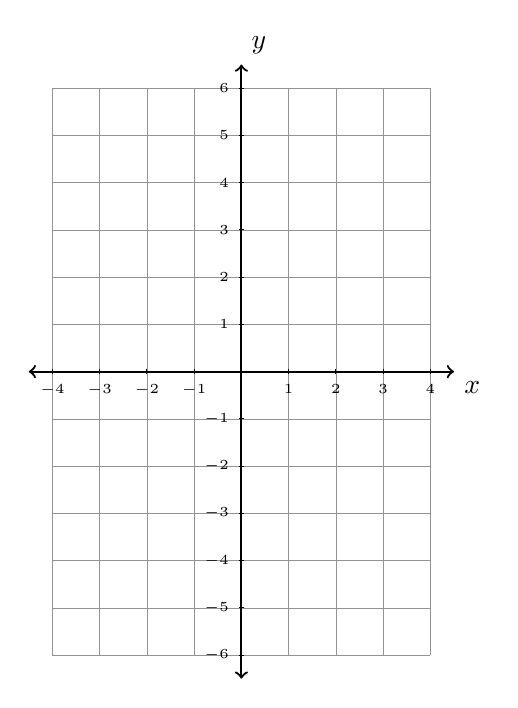
\begin{tikzpicture}[y=.6cm, x=.6cm,font=\sffamily,
	mydot/.style={
    circle,
    fill=white,
    draw,
    outer sep=0pt,
    inner sep=1.5pt
  }]
    %% Add a grid
    \draw[step = 1, gray, very thin,opacity=0.85] (-4, -6) grid (4, 6);
 	%% Draw the axes
	\draw[thick,<->] (-4.5,0) -- coordinate (x axis mid) (4.5,0) node[anchor = north west] {$x$};
    \draw[thick,<->] (0,-6.5) -- coordinate (y axis mid) (0,6.5) node[anchor = south west] {$y$};
    %% Label the y axis
    \foreach \y in {-6,...,-1,1,2,...,6} {
      \draw (1pt, \y) -- (-1pt, \y) node[anchor =  east] {\tiny$\y$};
    }
    %% Label the x axis
    \foreach \x in {-4,...,-1,1,2,...,4} {
      \draw (\x,1pt) -- (\x,-1pt) node[anchor = north] {\tiny$\x$};
    }

  \end{tikzpicture}

  \end{minipage}
\end{tabular}

\vfill


\item $\displaystyle g(x)=\left(\frac{1}{3}\right)^x$

  \begin{tabular}{ll}
    \begin{minipage}[t]{0.5\linewidth}
      \begin{enumerate}
      \item Shift 1 unit to the left.
      \item Stretch horizontally by a factor of 4.
      \item Reflect across the $x$-axis.
      \end{enumerate}
    \end{minipage}

    &
              
      \begin{minipage}[m]{0.5\linewidth}
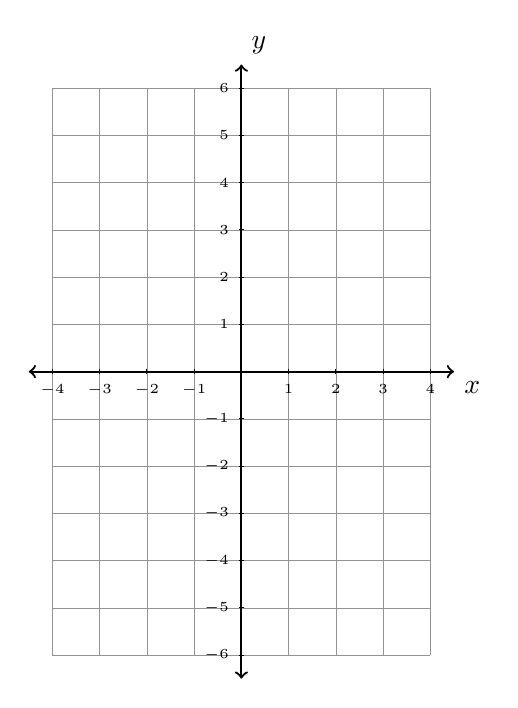
\begin{tikzpicture}[y=.6cm, x=.6cm,font=\sffamily,
	mydot/.style={
    circle,
    fill=white,
    draw,
    outer sep=0pt,
    inner sep=1.5pt
  }]
    %% Add a grid
    \draw[step = 1, gray, very thin,opacity=0.85] (-4, -6) grid (4, 6);
 	%% Draw the axes
	\draw[thick,<->] (-4.5,0) -- coordinate (x axis mid) (4.5,0) node[anchor = north west] {$x$};
    \draw[thick,<->] (0,-6.5) -- coordinate (y axis mid) (0,6.5) node[anchor = south west] {$y$};
    %% Label the y axis
    \foreach \y in {-6,...,-1,1,2,...,6} {
      \draw (1pt, \y) -- (-1pt, \y) node[anchor =  east] {\tiny$\y$};
    }
    %% Label the x axis
    \foreach \x in {-4,...,-1,1,2,...,4} {
      \draw (\x,1pt) -- (\x,-1pt) node[anchor = north] {\tiny$\x$};
    }

  \end{tikzpicture}
  \end{minipage}
      
  \end{tabular}


\vfill


\end{enumerate}

\clearpage
\subsection{Solving Exponential Equations}
Solving an equation means to find the set of values that can be
substituted for the variable, creating a true statement.


\textbf{Example.} To solve the equation, $\sqrt[3]{x}=3$ we need to
undo the operations happening to $x$.  Remember,
$\sqrt[3]{x}=x^{1/3}$.

\begin{equation*}
  \begin{array}{rcl@{\hspace{2em}}l}
    x^{1/3} & = & 3 & \textrm{Original~equation.}\\
    \left(x^{1/3}\right)^{3/1} & = & 3^{3/1} & \textrm{Raise~both~sides~to~$3/1$.}\\
    x^1 & = & 3^3 & \textrm{Use~exponential~properties.} \\
    x & = & 27    & \textrm{Simplify.}
  \end{array}
\end{equation*}

\item Use the example above to solve each of the following
  equations. Take one step at a time and write down each step.
\begin{enumerate}
\item  $x^{3/2}=64$. 
  \vfill
\item  $5x^{1/7}-2=13$
  \vfill
\end{enumerate}




\clearpage
\subsection{Compound Interest}


\noindent The compound interest formula is
$$A(t)=P\left(1+\frac{r}{n}\right) ^{nt},$$
where $P$ is the initial principal, $r$ is the annual compounded
interest rate (a number between 0 and 1), $n$ is the number of
compounding periods per year, and $t$ is the time in years.

\item If \$10,000 is invested at an annual rate of 8\%, determine the
  amount present after 10 years given the following:

\begin{enumerate}
\item Compounded annually\vfill
\item Compounded monthly \vfill
\item Compounded weekly \vfill
\item Compounded daily \vfill
\item Compounded hourly \vfill
\item Compounded every minute \vfill
\item Compounded continuously\vfill
\end{enumerate}

What is the general trend, and how do the results relate to one
another?

\clearpage

\subsection{Laws of Exponents} ~

\noindent
\fbox{
  \parbox{\dimexpr 0.6\linewidth}%
  {
    \noindent
    Laws of Exponents \\
    \begin{equation*}
      \begin{array}{rcl@{\hspace{4em}}rcl}
        a^m \cdot a^n & = & a^{m+n}  & \left(\dfrac{a}{b}\right)^n & = & \dfrac{a^n}{b^n} \\ [20pt]
        (a^m)^n & = & a^{mn}  &  \dfrac{a^m}{a^n} & = & a^{m-n} \\ [20pt]
        (ab)^n & = & a^nb^n &  \dfrac{1}{a^n} & = & a^{-n}
      \end{array}
    \end{equation*}
  }
}



\item Simplify the expressions completely (there should only be one
  instance of each variable and only positive exponents). For each
  step, identify the rule used to simplify.

\begin{enumerate}
\item $\left(\dfrac{x}{y}\right)^{-9}\cdot y^{10}$

  \vfill

\item $\left(-2x^3y\right)^5 \left(\dfrac{x^9}{5y^2}\right)$

  \vfill

\item $\dfrac{\sqrt{x^4y^3}}{y}$

  \vfill

\item $\sqrt{x^2+4}$

  \vfill

\end{enumerate}


%\clearpage
%
%\item  Match the following functions to their graph.
%
%\begin{multicols}{4}
%\begin{enumerate}
%	\item $y=2^x$
%	\item $y=1.25^x$
%	\item $y=-2^x$
%	\item $y=-1.25^x$
%	\item $y=2^{-x}$
%	\item $y=1.25^{-x}$
%	\item $y=-2^{-x}$
%	\item $y=-1.25^{-x}$
%\end{enumerate}	
%\end{multicols}
%
%
%\begin{center}
%\begin{tikzpicture}[y=.8cm, x=.8cm,font=\sffamily,
%	mydot/.style={
%    circle,
%    fill=white,
%    draw,
%    outer sep=0pt,
%    inner sep=1.5pt
%  }]
%    %% Add a grid
%    \draw[step = 1, gray, very thin,opacity=0.85] (-8, -8) grid (8, 8);
% 	%% Draw the axes
%	\draw[thick,<->] (-8.5,0) -- coordinate (x axis mid) (8.5,0) node[anchor = north west] {$x$};
%    \draw[thick,<->] (0,-8.5) -- coordinate (y axis mid) (0,8.5) node[anchor = south west] {$y$};
%    %% Label the y axis
%    \foreach \y in {-8,...,-1,1,2,...,8} {
%      \draw (1pt, \y) -- (-1pt, \y) node[anchor = south east] {\tiny $\y$};
%    }
%    %% Label the x axis
%    \foreach \x in {-8,...,-1,1,2,...,8} {
%      \draw (\x,1pt) -- (\x,-1pt) node[anchor = north] {\tiny $\x$};
%    }
%    %% Draw the function.
%    \begin{scope}
%%         \draw[very thick,blue] (-3,2) -- (1,1);
%%         \draw[very thick,blue] (3.05,1.05) -- (4,3);
%%         \draw[very thick,blue] (1.1,4) -- (3,4);
%    %semi-circle
%         %\draw[very thick, blue] (1,1) arc [radius=1, start angle=180, end angle= 5];
%     %parabola
%         %\draw[ultra thick, blue, domain=-5:0] plot (\x, {(-0.2)*(\x-5)*(\x+5)});
%         \draw[ultra thick, blue, <->, domain=-7.75:3.0] plot[samples=100] (\x, {2^\x});
%         \draw[ultra thick, red, <->, domain=-7.75:7.75] plot[samples=100] (\x, {(1.25)^\x});
%         \draw[ultra thick, orange, <->, domain=-3.0:7.75] plot[samples=100] (\x, {2^-\x});
%         \draw[ultra thick, purple, <->, domain=-7.75:7.75] plot[samples=100] (\x, {(1.25)^-\x});
%         \draw[ultra thick, blue, <->, domain=-3.0:7.75] plot[samples=100] (\x, {-2^-\x});
%         \draw[ultra thick, red, <->, domain=-7.75:7.75] plot[samples=100] (\x, {-(1.25)^-\x});
%         \draw[ultra thick, orange, <->, domain=-7.75:3.0] plot[samples=100] (\x, {-2^\x});
%         \draw[ultra thick, purple, <->, domain=-7.75:7.75] plot[samples=100] (\x, {-(1.25)^\x});
%           %dots
%%         \fill[blue] (-3, 2) circle[radius=0.5ex];
%%         \fill[blue] (1,1) circle[radius=0.5ex];
%%         \fill[blue] (4,3) circle[radius=0.5ex];
%%         \draw[very thick, blue] (3,1) circle[radius=0.5ex];
%%         \fill[blue] (3,4) circle[radius=0.5ex];
%%         \draw[very thick, blue] (1,4) circle[radius=0.5ex];
%
%
%    \end{scope}
%
%    %%\node[above=0.1cm] at (-2,2 )   {\nextXValue};
%
%\end{tikzpicture}
%\end{center}




\end{enumerate}


\hwTitle{Section 3.2}

\begin{enumerate}
\item Solve each of the following equations for $x$.
  \begin{enumerate}
  \item Solve the equation $x^{3/2}=8$
  \item Solve the equation $x^{2/3}=16$
  \item Solve the equation $x^{5/9}=243$
  \end{enumerate}
\item Simplify the expressions completely (there should only be one
  instance of each variable and only positive exponents). For each
  step, identify the rule used to simplify.
  \begin{enumerate}
  \item $\dfrac{x^{8/3}y^{3/5}}{x^2}$
  \item $\left( \dfrac{-2x^{-3}}{y^{12} }  \right)^{2/5}$
  \item $x^3 \cdot (2x)^2$
  \item $\dfrac{(\sqrt{x}(x-1))^{100} \cdot x^2}{(x-1)^{101}}$ 
  \item $\sqrt{x^2}$
  \end{enumerate}
\end{enumerate}


\preClass{Coordinate Systems}



\noindent Watch the Pre-Class videos for Section 3.3 and answer the following questions. Remember that in your written work you are graded on the correctness of your supporting work and not just your final answer. Always give an exact answer unless you are explicitly told to round; calculator approximations will not receive full credit. 


\begin{enumerate}
\item  Write the following in exponential form.
\begin{enumerate}
\item $\log_8(1)=0$
\vfill
\item $\ln(a)=b$
\vfill
\end{enumerate}


\item  Write the following in logarithmic form.
\begin{enumerate}
\item $7^0=1$
\vfill
\item $10^3=1000$
\vfill
\end{enumerate}

\item  Determine the domain of $\log_7(2x+5)$.  Write your answer in interval notation.
\vfill
\vfill

\newpage
\item  Graph the following functions.
\begin{enumerate}

\item Graph $\displaystyle f(x)=e^x$ along with it's asymptote.  (It is helpful to plot values for $x=0, 1, -1$.)\\
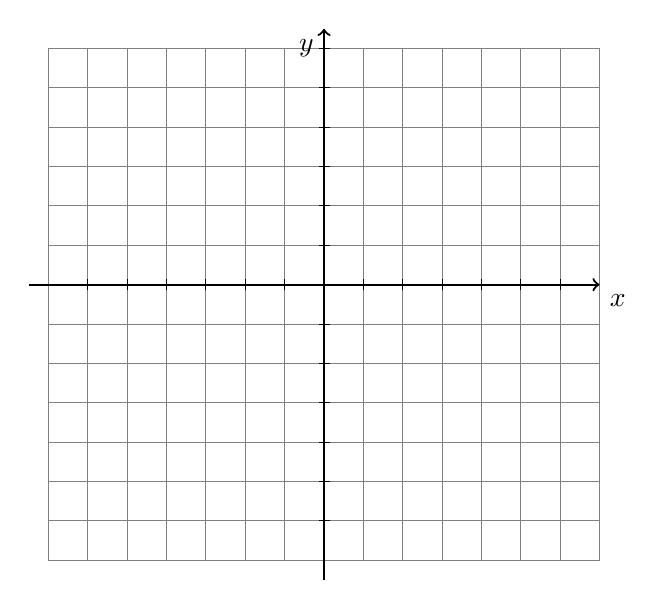
\begin{tikzpicture}[y=.5cm, x=0.5cm,font=\sffamily]
    %% ticks
    \draw[step = 1, gray] (-7,-7) grid (7,6);
    %% axis
    \draw[thick,->] (-7.5,0) -- coordinate (x axis mid) (7,0) node[anchor = north west] {$x$};
    \draw[thick,->] (0,-7.5) -- coordinate (y axis mid) (0,6.5) node[anchor = north east] {$y$};
    \foreach \y in {-6,-5,...,-1,1,2,...,6} {
      \draw (2pt, \y) -- (-2pt, \y);
    }
    \foreach \x in {-6,-5,...,-1,1,2,...,6} {
      \draw (\x,2pt) -- (\x,-2pt);
    }

\end{tikzpicture}



\item Use part $(a)$ to graph $\displaystyle g(x)=\ln(x)$ along with it's asymptote.\\

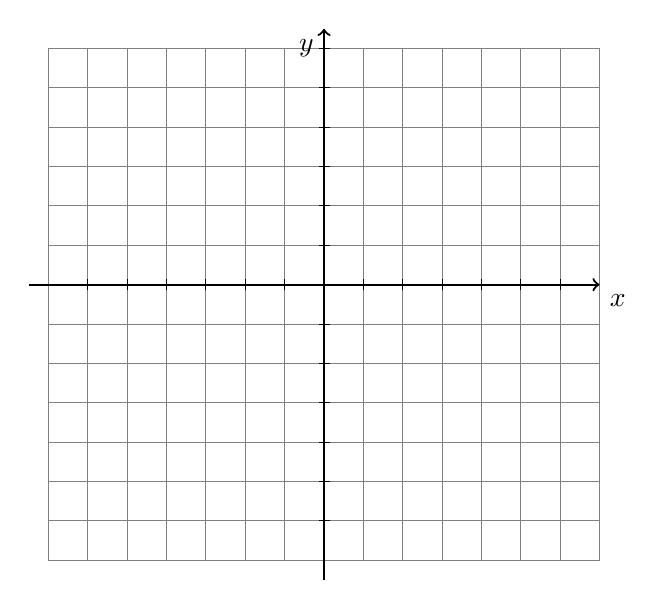
\begin{tikzpicture}[y=.5cm, x=0.5cm,font=\sffamily]
    %% ticks
    \draw[step = 1, gray] (-7,-7) grid (7,6);
    %% axis
    \draw[thick,->] (-7.5,0) -- coordinate (x axis mid) (7,0) node[anchor = north west] {$x$};
    \draw[thick,->] (0,-7.5) -- coordinate (y axis mid) (0,6.5) node[anchor = north east] {$y$};
    \foreach \y in {-6,-5,...,-1,1,2,...,6} {
      \draw (2pt, \y) -- (-2pt, \y);
    }
    \foreach \x in {-6,-5,...,-1,1,2,...,6} {
      \draw (\x,2pt) -- (\x,-2pt);
    }

\end{tikzpicture}


\vfill


\end{enumerate}






\end{enumerate}






\actTitle{Worksheet 3.3}


\noindent \textbf{Instructions:} Work together in groups of 3 or 4 to
complete the following problems.

Student goals:
  \begin{itemize}
  \item Use the logarithm function to solve for a variable in an
    equation that has exponential terms.
  \item Determine the domain and range of a simple function that
    contains logarithmic terms.
  \item Determine the inverse of a simple exponential function.
  \item Determine the inverse of a function that contains logarithmic terms.
  \item Graph basic logarithmic functions.
  \item Solve for a variable in a simple equation that contains logarithmic
    terms.
  %\item Recognize that $\log(x)=\log_{10}(x)$.
  %\item Recognize that $\ln(x)=\log_e(x)$.
  \end{itemize}



\begin{enumerate}
\item Write each of the following functions in their equivalent  exponential forms.
  $$\log_3(x)=9,   \quad \quad \quad \quad
  \log_2(8)=x,     \quad \quad \quad \quad
  \log_2(y)=5,     \quad \quad  \quad \quad
  \log_5(y)=2.$$
\vfill
\item Write each of the following functions in their equivalent  logarithmic forms.
  $$y=3^4,  \quad \quad \quad \quad \quad \quad
  m=4^2,    \quad \quad \quad \quad \quad \quad
  64=4^x,   \quad \quad \quad \quad  \quad \quad
  32=x^5.$$
\vfill
\item Solve each of the following expressions for the unknown value by
  first rewriting the equation in exponential form.
\begin{enumerate}
\item $\log_3(x)=4$
\vfill
\vfill
\item $\log_{m}(81)=4$
\vfill
\vfill
\item $\displaystyle \log_2\left(\frac{x}{2}\right)=5$
\vfill
\vfill
\end{enumerate}



\clearpage
\item Determine the inverse of each of the following functions.
  (Hint: rewrite each expression in logarithmic or exponential form
  after switching $x$ and $y$.)  Determine the domain and range of the
  function and its inverse.
\begin{enumerate}
\item $f(x)=\log_3(x)$

  \vfill
  
  \begin{tabular}{p{0.5\textwidth}p{0.5\textwidth}}
    $f^{-1}(x) = $ & \\ [1em]
    Domain of $f(x)$:  & Domain of $f^{-1}(x)$: \\ [1em]
    Range of $f(x)$:   & Range of $f^{-1}(x)$:  \\ [1em]
  \end{tabular}
  
\item $g(x)=\log_5(x+3)$

  \vfill
  
  \begin{tabular}{p{0.5\textwidth}p{0.5\textwidth}}
    $g^{-1}(x) = $ & \\ [1em]
    Domain of $g(x)$:  & Domain of $g^{-1}(x)$: \\ [1em]
    Range of $g(x)$:   & Range of $g^{-1}(x)$:  \\ [1em]
  \end{tabular}
  
\item $p(x)=e^{3x}$

  \vfill
  
  \begin{tabular}{p{0.5\textwidth}p{0.5\textwidth}}
    $p^{-1}(x) = $ & \\ [1em]
    Domain of $p(x)$:  & Domain of $p^{-1}(x)$: \\ [1em]
    Range of $p(x)$:   & Range of $p^{-1}(x)$:  \\ [1em]
  \end{tabular}

\end{enumerate}

\clearpage
  
\item Graph $q(x)=2^x$ and $q^{-1}(x)=\log_2(x)$ on the rectangular
  coordiantes below. Also, graph and label their asymptotes.

\begin{itemize}
\begin{multicols}{2}
\item[(a)] $q(x)=2^x$

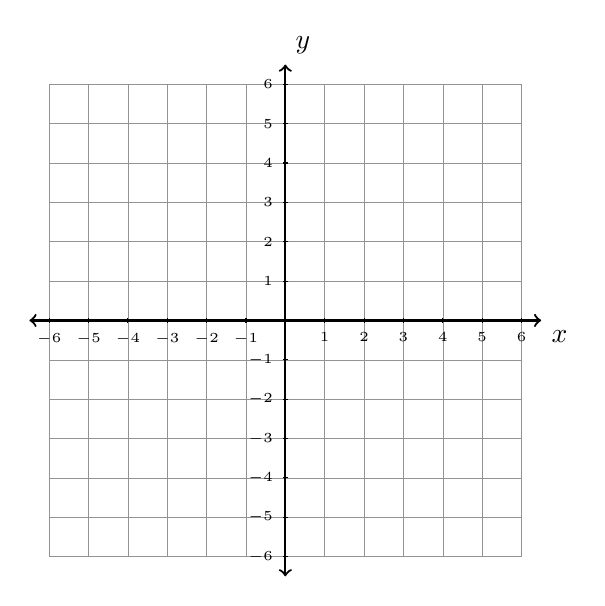
\begin{tikzpicture}[y=.5cm, x=.5cm,font=\sffamily,
	mydot/.style={
    circle,
    fill=white,
    draw,
    outer sep=0pt,
    inner sep=1.5pt
  }]
    %% Add a grid
    \draw[step = 1, gray, very thin,opacity=0.85] (-6, -6) grid (6, 6);
 	%% Draw the axes
	\draw[thick,<->] (-6.5,0) -- coordinate (x axis mid) (6.5,0) node[anchor = north west] {$x$};
    \draw[thick,<->] (0,-6.5) -- coordinate (y axis mid) (0,6.5) node[anchor = south west] {$y$};
    %% Label the y axis
    \foreach \y in {-6,...,-1,1,2,...,6} {
      \draw (1pt, \y) -- (-1pt, \y) node[anchor =  east] {\tiny$\y$};
    }
    %% Label the x axis
    \foreach \x in {-6,...,-1,1,2,...,6} {
      \draw (\x,1pt) -- (\x,-1pt) node[anchor = north] {\tiny$\x$};
    }
    %% Draw the function.
 %   \begin{scope}
 %        \draw[very thick,black] (-3,2) -- (1,1);
 %        \draw[very thick,black] (3.05,1.05) -- (4,3);
    %semi-circle
  %       \draw[very thick, black] (1,1) arc [radius=1, start angle=180, end angle= 5];
     %parabola
     %    \draw[ultra thick, black, domain=-5:0] plot (\x, {(-0.2)*(\x-5)*(\x+5)});
     %dots
     %  \fill[black] (-3, 2) circle[radius=0.5ex];
     %   \fill[black] (1,1) circle[radius=0.5ex];
     %    \fill[black] (4,3) circle[radius=0.5ex];
     %     \draw[very thick, black] (3,1) circle[radius=0.5ex];


   % \end{scope}

    %%\node[above=0.1cm] at (-2,2 )   {\nextXValue};

  \end{tikzpicture}

\vspace{1in}


\item[(b)] $q^{-1}(x)=\log_2(x)$ 

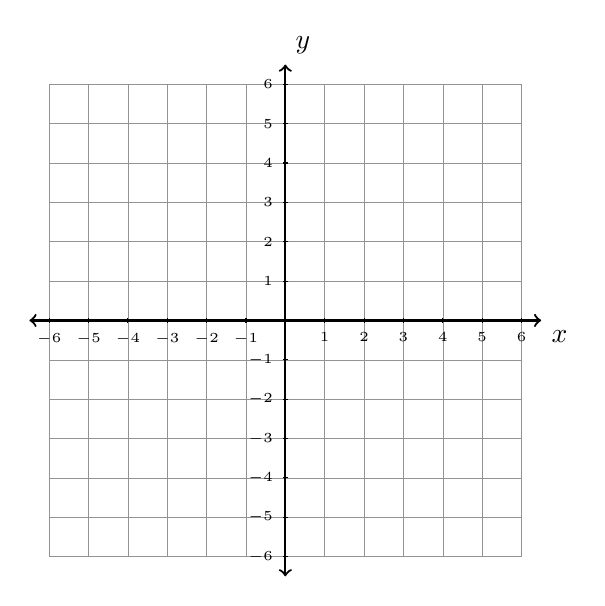
\begin{tikzpicture}[y=.5cm, x=.5cm,font=\sffamily,
	mydot/.style={
    circle,
    fill=white,
    draw,
    outer sep=0pt,
    inner sep=1.5pt
  }]
    %% Add a grid
    \draw[step = 1, gray, very thin,opacity=0.85] (-6, -6) grid (6, 6);
 	%% Draw the axes
	\draw[thick,<->] (-6.5,0) -- coordinate (x axis mid) (6.5,0) node[anchor = north west] {$x$};
    \draw[thick,<->] (0,-6.5) -- coordinate (y axis mid) (0,6.5) node[anchor = south west] {$y$};
    %% Label the y axis
    \foreach \y in {-6,...,-1,1,2,...,6} {
      \draw (1pt, \y) -- (-1pt, \y) node[anchor =  east] {\tiny$\y$};
    }
    %% Label the x axis
    \foreach \x in {-6,...,-1,1,2,...,6} {
      \draw (\x,1pt) -- (\x,-1pt) node[anchor = north] {\tiny$\x$};
    }
    %% Draw the function.
 %   \begin{scope}
 %        \draw[very thick,black] (-3,2) -- (1,1);
 %        \draw[very thick,black] (3.05,1.05) -- (4,3);
    %semi-circle
  %       \draw[very thick, black] (1,1) arc [radius=1, start angle=180, end angle= 5];
     %parabola
     %    \draw[ultra thick, black, domain=-5:0] plot (\x, {(-0.2)*(\x-5)*(\x+5)});
     %dots
     %  \fill[black] (-3, 2) circle[radius=0.5ex];
     %   \fill[black] (1,1) circle[radius=0.5ex];
     %    \fill[black] (4,3) circle[radius=0.5ex];
     %     \draw[very thick, black] (3,1) circle[radius=0.5ex];


   % \end{scope}

    %%\node[above=0.1cm] at (-2,2 )   {\nextXValue};

  \end{tikzpicture}


\end{multicols}
\end{itemize}


\item Graph each of the following transformed logarithmic functions.  

\begin{itemize}

\item[(a)] $m(x)=\log_2(-x+3)+1$

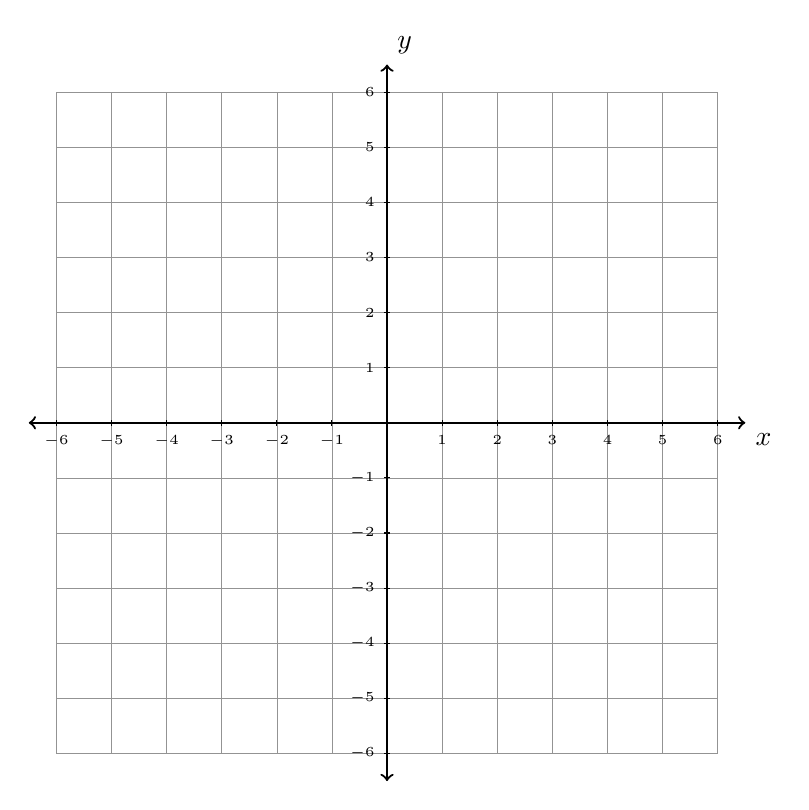
\begin{tikzpicture}[y=.7cm, x=.7cm,font=\sffamily,
	mydot/.style={
    circle,
    fill=white,
    draw,
    outer sep=0pt,
    inner sep=1.5pt
  }]
    %% Add a grid
    \draw[step = 1, gray, very thin,opacity=0.85] (-6, -6) grid (6, 6);
 	%% Draw the axes
	\draw[thick,<->] (-6.5,0) -- coordinate (x axis mid) (6.5,0) node[anchor = north west] {$x$};
    \draw[thick,<->] (0,-6.5) -- coordinate (y axis mid) (0,6.5) node[anchor = south west] {$y$};
    %% Label the y axis
    \foreach \y in {-6,...,-1,1,2,...,6} {
      \draw (1pt, \y) -- (-1pt, \y) node[anchor =  east] {\tiny$\y$};
    }
    %% Label the x axis
    \foreach \x in {-6,...,-1,1,2,...,6} {
      \draw (\x,1pt) -- (\x,-1pt) node[anchor = north] {\tiny$\x$};
    }
    %% Draw the function.
 %   \begin{scope}
 %        \draw[very thick,black] (-3,2) -- (1,1);
 %        \draw[very thick,black] (3.05,1.05) -- (4,3);
    %semi-circle
  %       \draw[very thick, black] (1,1) arc [radius=1, start angle=180, end angle= 5];
     %parabola
     %    \draw[ultra thick, black, domain=-5:0] plot (\x, {(-0.2)*(\x-5)*(\x+5)});
     %dots
     %  \fill[black] (-3, 2) circle[radius=0.5ex];
     %   \fill[black] (1,1) circle[radius=0.5ex];
     %    \fill[black] (4,3) circle[radius=0.5ex];
     %     \draw[very thick, black] (3,1) circle[radius=0.5ex];


   % \end{scope}

    %%\node[above=0.1cm] at (-2,2 )   {\nextXValue};

  \end{tikzpicture}

\vspace{1in}


\item[(b)] $w^{-1}(x)=2\log_3(x+4)-1$ 

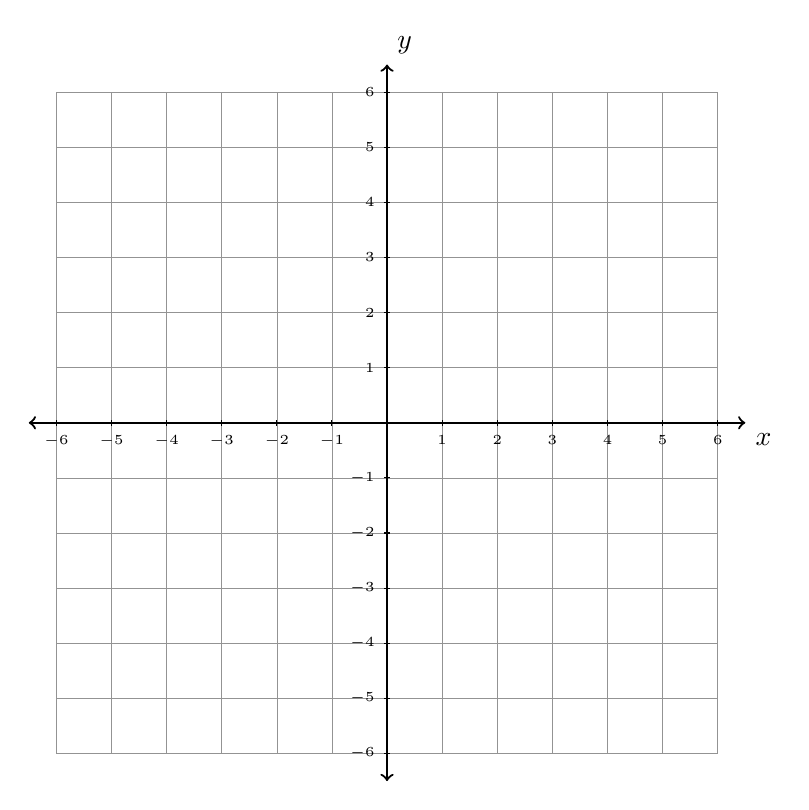
\begin{tikzpicture}[y=.7cm, x=.7cm,font=\sffamily,
	mydot/.style={
    circle,
    fill=white,
    draw,
    outer sep=0pt,
    inner sep=1.5pt
  }]
    %% Add a grid
    \draw[step = 1, gray, very thin,opacity=0.85] (-6, -6) grid (6, 6);
 	%% Draw the axes
	\draw[thick,<->] (-6.5,0) -- coordinate (x axis mid) (6.5,0) node[anchor = north west] {$x$};
    \draw[thick,<->] (0,-6.5) -- coordinate (y axis mid) (0,6.5) node[anchor = south west] {$y$};
    %% Label the y axis
    \foreach \y in {-6,...,-1,1,2,...,6} {
      \draw (1pt, \y) -- (-1pt, \y) node[anchor =  east] {\tiny$\y$};
    }
    %% Label the x axis
    \foreach \x in {-6,...,-1,1,2,...,6} {
      \draw (\x,1pt) -- (\x,-1pt) node[anchor = north] {\tiny$\x$};
    }
    %% Draw the function.
 %   \begin{scope}
 %        \draw[very thick,black] (-3,2) -- (1,1);
 %        \draw[very thick,black] (3.05,1.05) -- (4,3);
    %semi-circle
  %       \draw[very thick, black] (1,1) arc [radius=1, start angle=180, end angle= 5];
     %parabola
     %    \draw[ultra thick, black, domain=-5:0] plot (\x, {(-0.2)*(\x-5)*(\x+5)});
     %dots
     %  \fill[black] (-3, 2) circle[radius=0.5ex];
     %   \fill[black] (1,1) circle[radius=0.5ex];
     %    \fill[black] (4,3) circle[radius=0.5ex];
     %     \draw[very thick, black] (3,1) circle[radius=0.5ex];


   % \end{scope}

    %%\node[above=0.1cm] at (-2,2 )   {\nextXValue};

  \end{tikzpicture}



\end{itemize}

\noindent
\fbox{
  \parbox{\dimexpr\linewidth}%
  {    
    Since $r(x)=b^x$ and $s(x)=\log_b(x)$ are inverses,
    $$ r(s(x))=b^{\log_b(x)}=x \quad \quad \quad \quad
    s(r(x))=\log_b(b^x)=x.$$
  }
}

\item Evaluate the following expressions.  \sideNote{Express each of
    the terms within the parenthesis in a form that will allow you to
    take advantage of the definition of the inverse.}
  \begin{enumerate}
  \item $\log_{10}\left(1000\right)=$
    \vfill
  \item $\log_3\left(27\right)=$
    \vfill
  \item $\log_4\left(1\right)=$
    \vfill
  \item $\displaystyle \log_2\left(\frac{1}{4}\right)=$
    \vfill
  \item $3^{\log_3\left(12\right)}=$
    \vfill
  \item $e^{\ln\left(4\right)}=$
    \vfill
  \item $64^{\log_4\left(2\right)}=$
    \vfill
  \end{enumerate}

  \clearpage

\item With the advent of high frequency stock trading new methods to
  quantify the volatility of a security have been devised. The idea is
  to take the time that securities are traded, and divide the time up
  into equal time periods. The trading day may be divided up into ten
  minute intervals, and the price of a security at the end of each
  time period is recorded. For example, the price of a stock at the
  end of the 50\textsuperscript{th} minute of the trading day would be
  designated as $P_5$. One proposed measure of volatility is to take
  the logarithm of the ratio of the prices between two successive time
  periods. The volatility of a stock from the 50\textsuperscript{th}
  to the 60\textsuperscript{th} minute of the day would be
  \begin{eqnarray*}
    V_6(t) & = & \ln\left(\frac{P_6}{P_5}\right).
  \end{eqnarray*}

  \begin{enumerate}
  \item Briefly describe what happens to the volatility, $V_6$, as
    $P_6$ gets bigger than $P_5$. How does the volatility change as
    $P_6$ gets much bigger?
    \vfill
  \item Briefly describe what happens to the volatility, $V_6$, as
    $P_6$ gets smaller than $P_5$. How does the volatility change as
    $P_6$ gets much smaller?
    \vfill
  \item Under what circumstances is the volatility, $V_6$, close to
    zero?
    \vfill
  \item If you purchase a security in the morning and monitor the
    volatility of the security throughout the day, do you prefer to
    see positive or negative numbers for the volatility? If the
    volatility gets bigger how does the price of the stock change?
    \vfill

  \item A different way to quantify volatility has been proposed using
    the following definition:
    \sideNote{What might happen when you add the volatilities of a security over successive time periods?}
    \begin{eqnarray*}
      \hat{V}_6(t) & = & \left(\ln\left(\frac{P_6}{P_5}\right)\right)^2.
    \end{eqnarray*}
    How is this different, and what are the relative advantages and
    disadvantages of the definition?
    \vfill

  \end{enumerate}
  
\end{enumerate}

\hwTitle{Section 3.3}
  
\begin{enumerate}
\item Solve each of the following expressions for the unknown value by
  first rewriting the equation in exponential form.
  \begin{enumerate}
  \item $\displaystyle \log_2(4x)=5$
  \item $\displaystyle \log_4\left(\sqrt{x}\right)=2$
  \item $\displaystyle \log_{a}(216)=3$
  \item $\displaystyle \log_2\left(x^5\right)=8$
  \end{enumerate}

\item Determine the inverse of each of the following functions.
  (Hint: rewrite each expression in logarithmic or exponential form
  after switching $x$ and $y$.)  Determine the domain and range of the
  function and its inverse.
  \begin{enumerate}
  \item $h(x)=\ln(7x-4)$,  \quad \quad \quad $h^{-1}(x)=$ \\
    \begin{flushright}
      \begin{tabular}{l@{\hspace{3em}}l}
        Domain of $h(x)$:  &  Range of $h(x)$: \\
        Domain of $h^{-1}(x)$:   & Range of $h^{-1}(x)$:
      \end{tabular}
    \end{flushright}
    \item $\displaystyle k(x)=4^{x+3}$  \quad \quad \quad $k^{-1}(x)=$
      \begin{flushright}
        \begin{tabular}{l@{\hspace{3em}}l}
          Domain of $k(x)$: & Range of $k(x)$: \\
          Domain of $k^{-1}(x)$:  &  Range of $k^{-1}(x)$:
        \end{tabular}
      \end{flushright}
  \end{enumerate}

\item Graph each of the following transformed logarithmic functions.  
\item[(c)] $u(x)=-3\ln(x-2)$

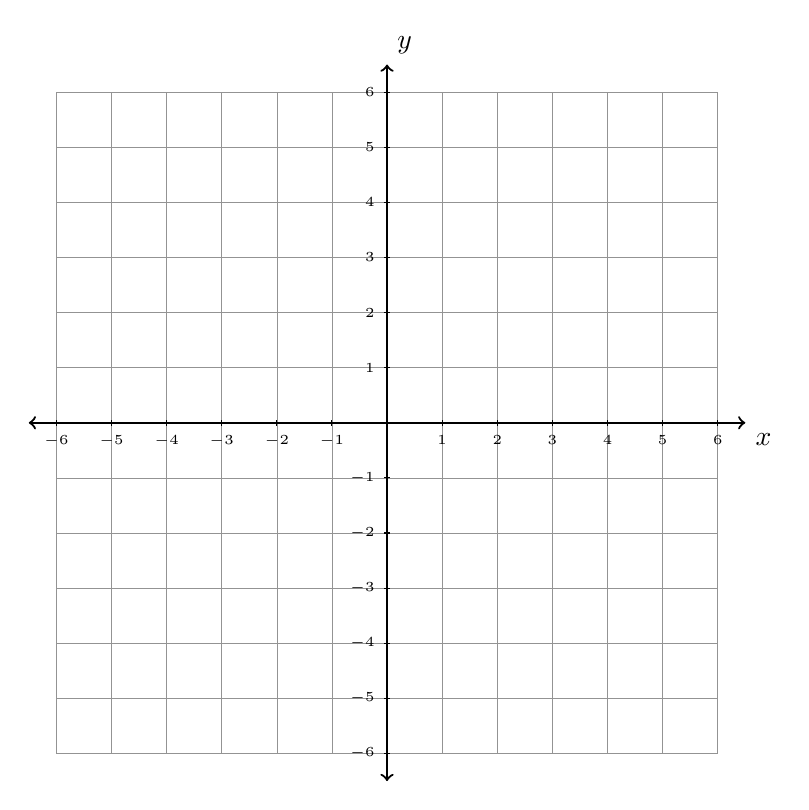
\begin{tikzpicture}[y=.7cm, x=.7cm,font=\sffamily,
	mydot/.style={
    circle,
    fill=white,
    draw,
    outer sep=0pt,
    inner sep=1.5pt
  }]
    %% Add a grid
    \draw[step = 1, gray, very thin,opacity=0.85] (-6, -6) grid (6, 6);
 	%% Draw the axes
	\draw[thick,<->] (-6.5,0) -- coordinate (x axis mid) (6.5,0) node[anchor = north west] {$x$};
    \draw[thick,<->] (0,-6.5) -- coordinate (y axis mid) (0,6.5) node[anchor = south west] {$y$};
    %% Label the y axis
    \foreach \y in {-6,...,-1,1,2,...,6} {
      \draw (1pt, \y) -- (-1pt, \y) node[anchor =  east] {\tiny$\y$};
    }
    %% Label the x axis
    \foreach \x in {-6,...,-1,1,2,...,6} {
      \draw (\x,1pt) -- (\x,-1pt) node[anchor = north] {\tiny$\x$};
    }
    %% Draw the function.
 %   \begin{scope}
 %        \draw[very thick,black] (-3,2) -- (1,1);
 %        \draw[very thick,black] (3.05,1.05) -- (4,3);
    %semi-circle
  %       \draw[very thick, black] (1,1) arc [radius=1, start angle=180, end angle= 5];
     %parabola
     %    \draw[ultra thick, black, domain=-5:0] plot (\x, {(-0.2)*(\x-5)*(\x+5)});
     %dots
     %  \fill[black] (-3, 2) circle[radius=0.5ex];
     %   \fill[black] (1,1) circle[radius=0.5ex];
     %    \fill[black] (4,3) circle[radius=0.5ex];
     %     \draw[very thick, black] (3,1) circle[radius=0.5ex];


   % \end{scope}

    %%\node[above=0.1cm] at (-2,2 )   {\nextXValue};

  \end{tikzpicture}

\vspace{1in}


\item[(d)] $v^{-1}(x)=\log_5(5-x)$ 

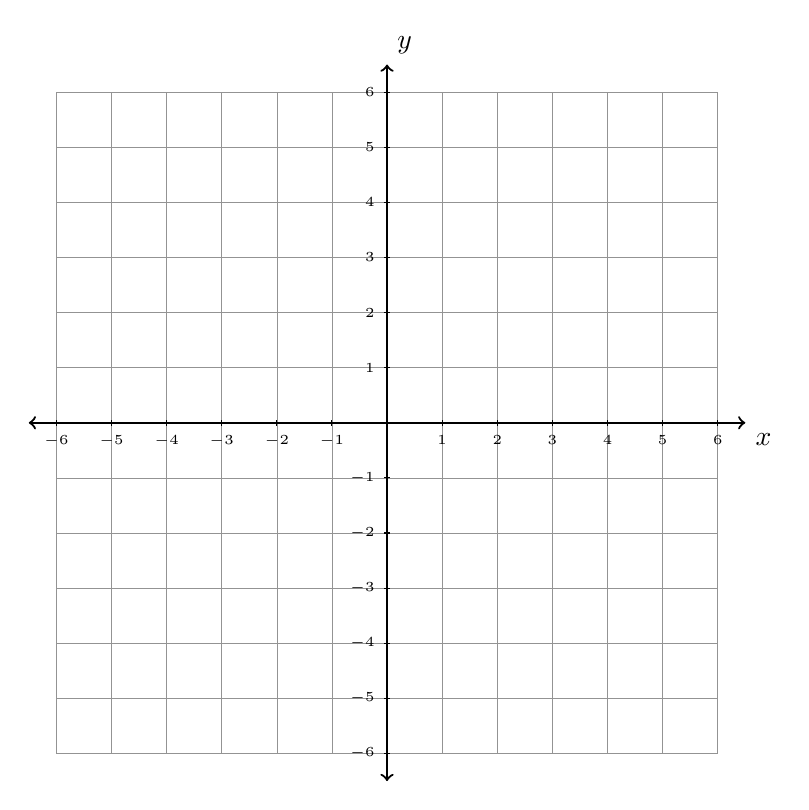
\begin{tikzpicture}[y=.7cm, x=.7cm,font=\sffamily,
	mydot/.style={
    circle,
    fill=white,
    draw,
    outer sep=0pt,
    inner sep=1.5pt
  }]
    %% Add a grid
    \draw[step = 1, gray, very thin,opacity=0.85] (-6, -6) grid (6, 6);
 	%% Draw the axes
	\draw[thick,<->] (-6.5,0) -- coordinate (x axis mid) (6.5,0) node[anchor = north west] {$x$};
    \draw[thick,<->] (0,-6.5) -- coordinate (y axis mid) (0,6.5) node[anchor = south west] {$y$};
    %% Label the y axis
    \foreach \y in {-6,...,-1,1,2,...,6} {
      \draw (1pt, \y) -- (-1pt, \y) node[anchor =  east] {\tiny$\y$};
    }
    %% Label the x axis
    \foreach \x in {-6,...,-1,1,2,...,6} {
      \draw (\x,1pt) -- (\x,-1pt) node[anchor = north] {\tiny$\x$};
    }
    %% Draw the function.
 %   \begin{scope}
 %        \draw[very thick,black] (-3,2) -- (1,1);
 %        \draw[very thick,black] (3.05,1.05) -- (4,3);
    %semi-circle
  %       \draw[very thick, black] (1,1) arc [radius=1, start angle=180, end angle= 5];
     %parabola
     %    \draw[ultra thick, black, domain=-5:0] plot (\x, {(-0.2)*(\x-5)*(\x+5)});
     %dots
     %  \fill[black] (-3, 2) circle[radius=0.5ex];
     %   \fill[black] (1,1) circle[radius=0.5ex];
     %    \fill[black] (4,3) circle[radius=0.5ex];
     %     \draw[very thick, black] (3,1) circle[radius=0.5ex];


   % \end{scope}

    %%\node[above=0.1cm] at (-2,2 )   {\nextXValue};

  \end{tikzpicture}

\item One way to change a logarithmic expression is to convert it into
  its logarithmic form and then back into its logarithmic form after
  performing some algebra steps. This can be difficult for non-trivial
  expressions. One particular example is examined:
  \begin{eqnarray*}
    y & = & \log(x) + \log(3).
  \end{eqnarray*}
  Show that the expression above is equivalent to $y=\log(3x)$ using
  the following steps:
  \begin{enumerate}
  \item Subtract $\log(3)$ from both sides.
  \item Substitute $u=y-\log(3)$.
  \item Rewrite the expression into its exponential form.
  \item Substitute the definition of $u$ so the new form is in terms of $y$.
  \item Use exponential properties and properties of the logarithm to show that
    \begin{eqnarray*}
      10^{y-\log(3)} & = & \frac{10^y}{3}.
    \end{eqnarray*}
    (Show all the steps required to establish this identity.)
  \item Solve the equation for $10^y$.
  \item Convert the new expression into its logarithmic form to show
    that $y=\log(3x)$.
  \end{enumerate}

\item Mimic the steps in the previous problem to show that
  $y=3\log(x)$ implies that $y=\log\left(x^3\right)$.

\end{enumerate}



\preClass{Coordinate Systems}



\noindent Watch the Pre-Class videos for Section 3.4 and answer the following questions. Remember that in your written work you are graded on the correctness of your supporting work and not just your final answer. Always give an exact answer unless you are explicitly told to round; calculator approximations will not receive full credit. 


\begin{enumerate}
\item Use logarithmic properties to simplify and condense the following into one logarithm.
\begin{enumerate}
\item $\ln(x)+\ln(y)-\ln(z)$
\vfill
\item $\displaystyle \log_2(x^2)+\frac{1}{2}\log_2(x-1)-3\log_2((x+3)^2)$
\vfill

\end{enumerate}


\item Use logarithmic properties to expand each expression.  
\begin{enumerate}
\item $\displaystyle \log_2\Big(\frac{x}{y^5}\Big)$
\vfill
\item $\displaystyle \ln \Big((y^2-16)(y+8)^2  \Big)$
\vfill

\end{enumerate}

\item (Use the change of base formula to approximate $\log_{7.5}(98)$ and round your answer to 4 decimal places.  Show all work.
\vfill







\end{enumerate}






\actTitle{Worksheet 3.4}


\noindent \textbf{Instructions:}  Work together in groups of  3 or 4 to complete the following problems.

\noindent CAUTION: There is NO RULE for breaking down $\log_a(u+w)$ or $\log_a(u-w)$.  

Student goals:
\begin{itemize}
\item Use the properties of logarithms to solve for a variable in a
  variety of more complex forms:
  \begin{eqnarray*}
    \log_a(u\cdot v) & = & \log_a(u) + \log_a(v), \\
    \log_a\left(\frac{u}{v}\right) & = & \log_a(u) - \log_a(v), \\
    \log_a\left(u^r\right) & = & r\log_a(u).
  \end{eqnarray*}
\item Solve for a variable when multiple logarithms with different
  bases are present in an expression.
\item Solve for a variable when multiple exponentials with different
  bases are present in an expression.
\end{itemize}

\hrule

\begin{enumerate}

\item Let $M=\log_b(x)$ and $N=\log_b(y)$.
\begin{enumerate}
\item Write the given equations in exponential form.

  \vfill
\item Show that $xy=b^{M+N}$.

  \vfill
\item Write the expression $xy=b^{M+N}$ in logarithmic form.

  \vfill

\item Substitute for $M$ and $N$.

  \vfill
  
\item What did you just show?

  \vspace{1em}

\end{enumerate}

\clearpage

\item Let $M=\log_b(x)$ and $N=\log_b(y)$.  Use the same process as
  that in the previous question to show the Quotient Property of
  Logarithms is true.
  $$\log_b\left(\frac{x}{y}\right)=\log_b(x)-\log_b(y)$$
\vfill
\vfill
\vfill


\clearpage

\item Expand the following to express in terms of logarithms of $x$, $y$, $z$, or $w$.
\begin{enumerate}
\item $\log_4(xz)$ \\[.2in]
%\item $\ln(\sqrt[7]{x^5})$
\item $\log_2\left( \dfrac{x}{y} \right)$ \\[.2in]
\item $\ln\left( \dfrac{w^2z^3}{y^2\sqrt[5]{x}} \right)$ \\[1in]
%\item $\log(z \sqrt[5]{x^7y^3})$
\end{enumerate}



\item Condense the following to express as a single logarithm.
\begin{enumerate}
%\item $\log_3(x)+\log_3(4y^2)$
\item $\log_7(4x^5)-\log_7(x^2)$ \\[.5in]
\item $-4\left(\ln(2)-\ln(7)\right)+5\ln(3)$ \\[.7in]
\item $7 \log_8 (x) - 3 \log_8(2x+3) + 2\log_8(x-3)$ \\[1in]
%\item  $\dfrac{1}{4} \ln(x y^2) + \dfrac{1}{3} \ln(y^5 \sqrt{x} )-3\ln\left(\dfrac{z}{y}\right)$

\end{enumerate}




\clearpage


\item Rewrite the function without using any logarithms.
\begin{enumerate}
\item $ \displaystyle f(x) = 10 \ln(e^{-7+2x})$ \\[.5in]
\item $\displaystyle f(x)=3^{\log_3(8)-5 \log_3(x^2+1)}$ \\[1in]

\item $f(x) = \log ({10}^{4x+y}{100}^{y-x})$ \\[1in]
\end{enumerate}


\item Use the given approximations to approximate the value of the following logarithms.
$$\log_b(2)\approx 0.356 \quad \quad \quad \quad \log_b(3)\approx 0.565 \quad \quad \quad \quad \log_b(5)\approx 0.827$$

\begin{enumerate}
\item $\log_b(15)$\vfill
\item $\log_b(10)$\vfill
\item $\log_b(81)$\vfill
\item $\displaystyle \log_b(\frac{15}{2})$\vfill
\end{enumerate}




\clearpage

\item  For each of the following functions, determine whether or not its graph is shown below.

\begin{multicols}{3}
\begin{enumerate}
	\item $y=2^x+3$
	\item $y=\ln(x-2)$
	\item $y = 2^{-x}+3$
	\item $y=e^{-x}-3$
	\item $y=-\ln(x-2)$
	\item $y=-\log_2(x+3)-4$
\end{enumerate}	
\end{multicols}


\begin{center}
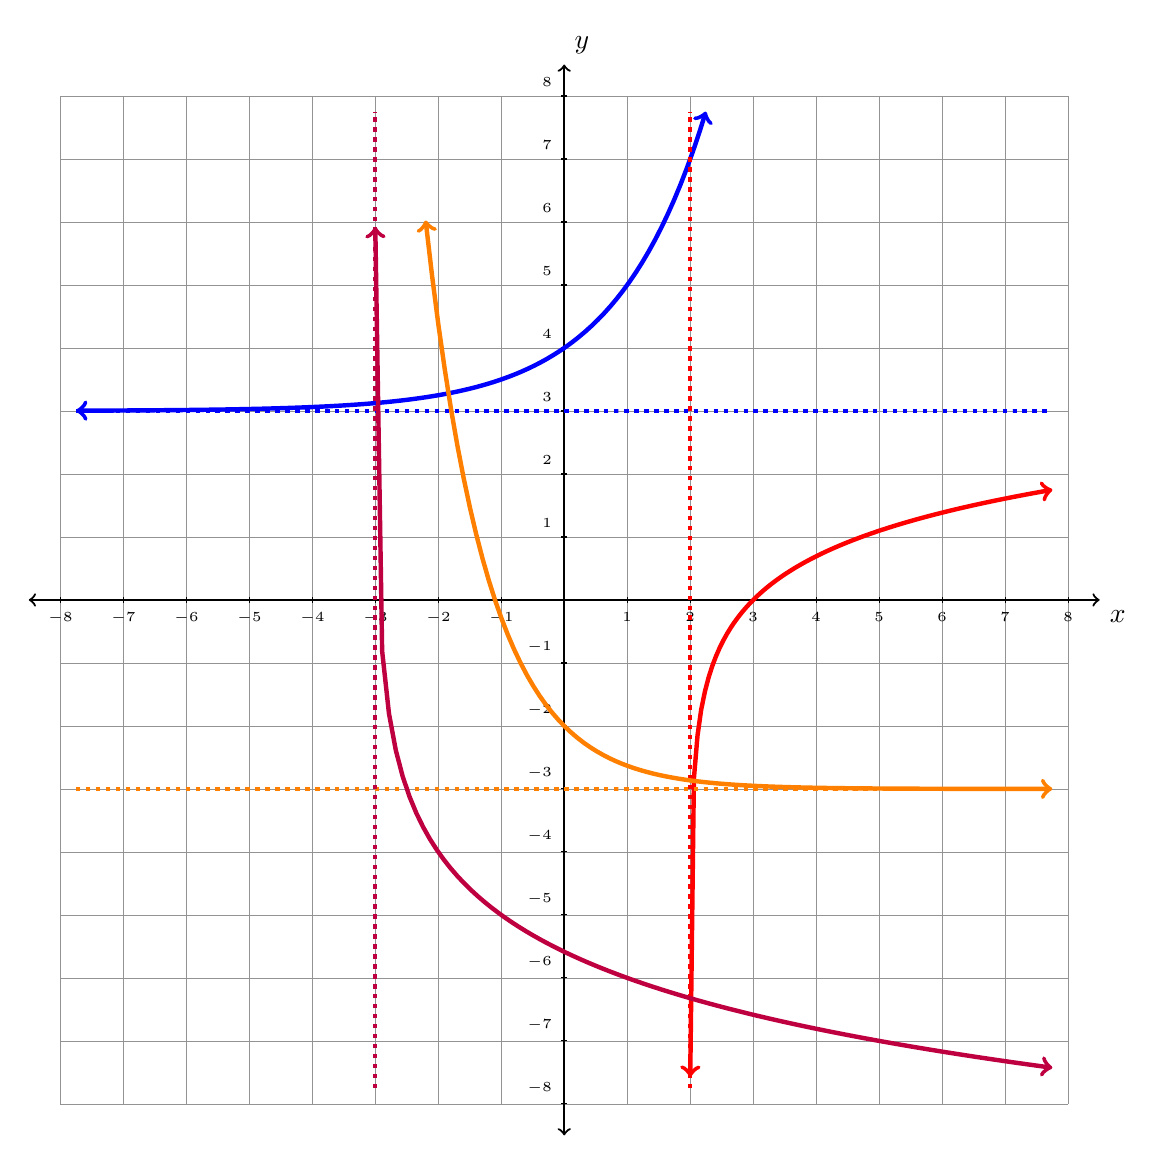
\begin{tikzpicture}[y=.8cm, x=.8cm,font=\sffamily,
	mydot/.style={
    circle,
    fill=white,
    draw,
    outer sep=0pt,
    inner sep=1.5pt
  }]
    %% Add a grid
    \draw[step = 1, gray, very thin,opacity=0.85] (-8, -8) grid (8, 8);
 	%% Draw the axes
	\draw[thick,<->] (-8.5,0) -- coordinate (x axis mid) (8.5,0) node[anchor = north west] {$x$};
    \draw[thick,<->] (0,-8.5) -- coordinate (y axis mid) (0,8.5) node[anchor = south west] {$y$};
    %% Label the y axis
    \foreach \y in {-8,...,-1,1,2,...,8} {
      \draw (1pt, \y) -- (-1pt, \y) node[anchor = south east] {\tiny $\y$};
    }
    %% Label the x axis
    \foreach \x in {-8,...,-1,1,2,...,8} {
      \draw (\x,1pt) -- (\x,-1pt) node[anchor = north] {\tiny $\x$};
    }
    %% Draw the function.
    \begin{scope}
%         \draw[very thick,blue] (-3,2) -- (1,1);
%         \draw[very thick,blue] (3.05,1.05) -- (4,3);
%         \draw[very thick,blue] (1.1,4) -- (3,4);
    %semi-circle
         %\draw[very thick, blue] (1,1) arc [radius=1, start angle=180, end angle= 5];
     %parabola
         %\draw[ultra thick, blue, domain=-5:0] plot (\x, {(-0.2)*(\x-5)*(\x+5)});
         \draw[ultra thick, blue, <->, domain=-7.75:2.25] plot[samples=100] (\x, {2^\x+3});
         \draw[ultra thick, blue, dotted, domain=-7.75:7.75] plot[samples=100] (\x, 3);
         \draw[ultra thick, red, <->, domain=2.0005:7.75] plot[samples=100] (\x, {ln(\x-2)});
         \draw[ultra thick, red, dotted, range=-7.75:7.75] plot[samples=100] (2,-7.75)--(2,7.75);
         \draw[ultra thick, orange, <->, domain=-2.2:7.75] plot[samples=100] (\x, {e^-\x-3});
         \draw[ultra thick, orange, dotted, domain=-7.75:7.75] plot[samples=100] (\x, -3);
         \draw[ultra thick, purple, <->, domain=-2.999:7.75] plot[samples=100] (\x, {-log2(\x+3)-4});
         \draw[ultra thick, purple, dotted, range=-7.75:7.75] plot[samples=100] (-3,-7.75)--(-3,7.75);

           %dots
%         \fill[blue] (-3, 2) circle[radius=0.5ex];
%         \fill[blue] (1,1) circle[radius=0.5ex];
%         \fill[blue] (4,3) circle[radius=0.5ex];
%         \draw[very thick, blue] (3,1) circle[radius=0.5ex];
%         \fill[blue] (3,4) circle[radius=0.5ex];
%         \draw[very thick, blue] (1,4) circle[radius=0.5ex];


    \end{scope}

    %%\node[above=0.1cm] at (-2,2 )   {\nextXValue};

\end{tikzpicture}
\end{center}





\item Use the change-of-base formula to write
  $\log_2(5)+\log_5(9)$ as a single
  logarithm using base $e$.

  \vfill




\end{enumerate}

\hwTitle{Section 3.4}




\actTitle{Worksheet 3.2-3.4 Review}

\noindent \textbf{Instructions:}  Work together in groups of  3 or 4 to complete the following problems.



\begin{enumerate}

\item Which functions are exponential functions?
$$f(x)=4.2^x \quad \quad g(x)=x^{4.2} \quad \quad h(x)=4.2x \quad \quad k(x)=(\sqrt{4.2})^x \quad \quad m(x)=(-4.2)^x$$

\item Consider $y=3^x$.  Determine the domain, range, and asymptote for each of the following functions.

\begin{enumerate}
\item $f(x)=3^x$\vfill
\item $g(x)=3^x+2$\vfill
\item $b(x)=3^{x+2}-1$\vfill


\item  $\displaystyle h(x)=\left(\frac{1}{3}\right)^x$
\vfill


\end{enumerate}

\item Alice will put \$15,000 into a savings account.  The first
  account offers an interest rate of 6.4\% compounded monthly. The
  second account offers an interest rate of 6.7\% compounded
  continuously.  Which option is best if the account will be left
  alone for five years. Is there a time when the choice will change?

\vfill
\vfill

\clearpage

\item Determine the domain, range, and asymptote for each of the following functions.
\begin{enumerate}
\item $f(x)=\log(8-x)$ 
\vfill
\item $g(x)=\log_2 (x^2-16)$ 
\vfill
\vfill
\item $h(x)=\ln(x^2+14)$
\vfill
\item $\displaystyle m(x)=3+\log_4\left(\frac{1}{\sqrt{11-x}}\right)$
\vfill
\end{enumerate}

\item Determine the domain of the following function and explain your answer. $$f(x)=\ln(-6x^2)$$
\vfill
\clearpage

\item Graph the function $f(x)=\log_{3}(x+2)+4$ along with it's asymptote.\\
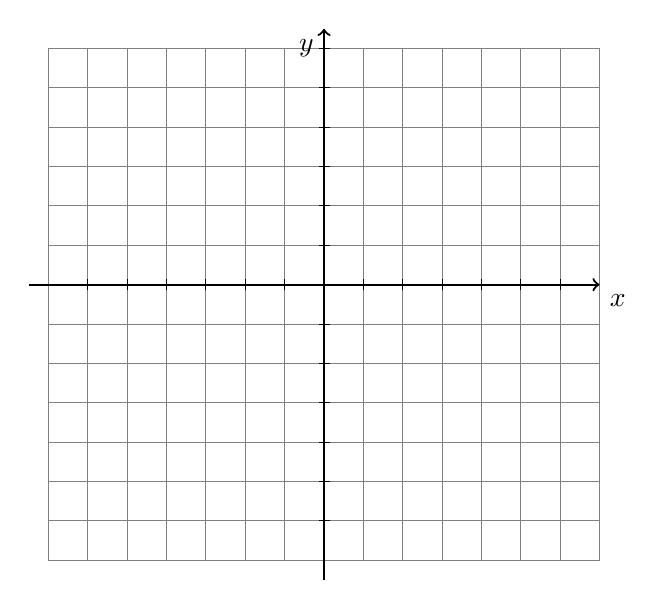
\begin{tikzpicture}[y=.5cm, x=0.5cm,font=\sffamily]
    %% ticks
    \draw[step = 1, gray] (-7,-7) grid (7,6);
    %% axis
    \draw[thick,->] (-7.5,0) -- coordinate (x axis mid) (7,0) node[anchor = north west] {$x$};
    \draw[thick,->] (0,-7.5) -- coordinate (y axis mid) (0,6.5) node[anchor = north east] {$y$};
    \foreach \y in {-6,-5,...,-1,1,2,...,6} {
      \draw (2pt, \y) -- (-2pt, \y);
    }
    \foreach \x in {-6,-5,...,-1,1,2,...,6} {
      \draw (\x,2pt) -- (\x,-2pt);
    }

\end{tikzpicture}


\vfill
\item Find a logarithmic function of the form $f(x)=b+\log_{a}(x+c)$ that has the vertical asymptote $x=-14$, passes through the point $(-13, 2)$ and crosses the $x$-axis at $x=\frac{-685}{49}$.
\vfill
\vfill
\vfill

\clearpage



\item Simplify the expression without using a calculator.
\begin{enumerate}

\item $\log_3(9)$\\

\item $\displaystyle \log_2(\frac{1}{16})$\\

\item $\log_{1/7}(49)$\\



\end{enumerate}







\item Simplify the expression without using a calculator.
\begin{enumerate}

\item $\displaystyle \log_4(4^{11})$\\

\item $\displaystyle 5^{\log_5(x+y)}$\\

\item $\log_{\pi}(1)$\\



\end{enumerate}






\item Write the logarithm as a sum or difference of logarithms and simplify as much as possible.  (Expand the logarithmic expression.)
\begin{enumerate}
\item $ \displaystyle \log_7\left(\frac{1}{7}mn^2\right)$ 
\vfill
\item $\displaystyle \log_5\left(\frac{p^5}{m\sqrt{n}}\right)$ 
\vfill

\item $\displaystyle \log\left(\frac{10}{\sqrt{a^2+b^2}}\right)$ 
\vfill

\item $\displaystyle \ln\left(\sqrt[5]{\frac{e^2}{c^2+5}}\right)$ 
\vfill


\end{enumerate}

\clearpage

\item Write the logarithmic expression as a single logarithm with coefficient 1, and simplify as much as possible.  (Condense the logarithmic expression.)


\begin{enumerate}
\item $\ln(y)+\ln(4)$\vfill
\item $\log_3(693)-\log_3(33)-\log_3(7)$\vfill
\item $3[\ln(x)-\ln(x+3)-\ln(x-3)]$\vfill
\item $\displaystyle 15\log(c)-\frac{1}{4}\log(d)-\frac{3}{4}\log(k)$\vfill
\end{enumerate}






\end{enumerate}




\preClass{Coordinate Systems}

\videoLink{Section 3.5 day 1 (parts 1-4)}{https://www.youtube.com/playlist?list=PLYHZK3b8UFw3bN2A-OphS45t9N4M0RDMM}


\begin{enumerate}
\item Solve the following equations.  Then check your answers.
\begin{enumerate}
\item $\displaystyle 4^{x+2}=64$
\vfill
\item $\ln(2x-3)=\ln(11)$
\vfill
\end{enumerate}


\item Solve the following equation.  Then check your answer.

 $$\displaystyle 5+e^{x+1}=20$$


\vfill
\vfill

\newpage

\item Solve the following equation.
$$3^x=4^{2x-5}$$



\end{enumerate}




\include{exponentials/Worksheet-3.5a}

\preClass{Coordinate Systems}


\videoLink{Section 3.5 day 2}{https://www.youtube.com/playlist?list=PLYHZK3b8UFw2U675u2QqFyf9AQlpZ6AZJ}

\begin{enumerate}
\item  Solve the following equations.  Then check your answers.  Leave your answers as symbolic expressions (no decimals).
\begin{enumerate}
\item $\displaystyle 5\log_6(7w+1)=10$
\vfill
\item $2\log_8(3y-5)+20=24$
\vfill


\end{enumerate}

\newpage

\item If \$10,000 is invested in an account earning 5.5\% interest compounded continuously, determine how long it will take for the money to triple.  Round your final answer to the nearest year.




\end{enumerate}




\include{exponentials/Worksheet-3.5b}

\preClass{Coordinate Systems}



\noindent Watch the Pre-Class videos for Section 3.6 and answer the following questions. Remember that in your written work you are graded on the correctness of your supporting work and not just your final answer. Always give an exact answer unless you are explicitly told to round; calculator approximations will not receive full credit. 


\begin{enumerate}
\item Suppose that \$50,000 from a retirement account is invested in a large cap stock fund.  After 20 years, the value is \$194,809.67.
\begin{enumerate}
\item Use the model $A=Pe^{rt}$ to determine the average rate of return under continuous compounding. (Do not simplify or round your answer.)
\vfill
\item  Assuming interest continues to accumulate at this average rate, how long will it take the investment to reach \$250,000?  Round your final answer to the nearest tenth of a year.
\vfill


\end{enumerate}

\newpage

\item  A sample from a mummified bull was taken from a pyramid in Dashur, Egypt.  The sample shows that 78\% of the carbon-14 still remains.  How old is the sample?  Round to the nearest year.  Use the model $Q(t)=Q_0e^{-0.000121t}$ for radiocarbon dating.



\end{enumerate}






\actTitle{Worksheet 3.6}


\noindent \textbf{Instructions:}  Work together in groups of  3 or 4
to complete the following problems.\\

Students should be able to do each of the following:
\begin{itemize}
\item Solve equations for various parameters.
\item Solve equations for a variable.
\item Construct equations from written descriptions.
\item Determine logistic relationships given a written description.
\item Identify growth vs decay given a verbal written description.
\end{itemize}

\noindent \textbf{NOTE 1:  }Half-life is the time it takes for 50\% (or half) of a substance to decay.\\
\noindent \textbf{NOTE 2:  }Leave all of your answers in symbolic form.


\begin{enumerate}


\item Determine which of the following are exponential \textbf{decay} functions.
$$f(t)=5^t \quad \quad \quad \quad g(t)=5^{-t}  \quad \quad \quad \quad h(t)=\left(\frac{1}{5}\right)^{t}  \quad \quad \quad \quad p(t)=\left(\frac{1}{5}\right)^{-t}$$



\item Carlos has taken an initial dose of a prescription medication.  The relationship between elapsed time $t$, in hours, since he took the first dose, and the amount of medication, $M(t)$, in milligrams (mg), in his bloodstream is modeled by the following function. $$M(t)=20e^{-0.8t}$$

\begin{enumerate}
\item  How much medication is in Carlos' bloodstream after 3 hours?\vfill
\item In how many hours will Carlos have 1 mg of medication remaining in his bloodstream?\vfill
\vfill
\end{enumerate}

\clearpage

\item You invest at 3\% per annum, compounded continuously.  Determine
  the time $t$ required for your investment to triple.

  \vfill


\item Money is invested at an interest rate of $r$ (where $r$ is a
  decimal) and is compounded continuously.  Express the time required
  for the money to triple, as a \textbf{function of $r$.}

  \vfill

\clearpage
  
\item The amount of a radioactive compound in a sample decays exponentially ($P=P_0e^{kt}$).  The sample initially contains 50g of the compound, and after three years contains 40g.  How long will it take until there is 30g of material?
\begin{enumerate}
\item Determine the two points $(t,P)$ given in the question.\\[.5in]
\item Use the two points in the given equation to determine the decay constant $k$.
\vfill
\item How long will it take until there is 30g of material?
\vfill
\item What is the half-life of the compound?\vfill
\end{enumerate}

\clearpage

\item The human population grew exponentially from 1.6 billion people in the year 1900 \\ to 6 billion in the year 2000.
\begin{enumerate}
\item If the population continues to grow at this rate, what will be the population in 2100? \\ To simplify calculations, I recommend using the year 1900 at year $t=0$.  Round your answer to the nearest tenth of a billion. \vfill \vfill
\item WOW! That is a lot of people!  \\ Suppose the population growth slows to follow the \textbf{logistic model} $$P=\dfrac{12}{1+22.3e^{-0.031t}}$$  where $P$ is measured in billions of people and $t$ in years since 1900. \\ In this model with reduced growth, what will be the population in 2100?  Round your answer to the nearest tenth of a billion. \vfill
\item Following the exponential growth, the population will continue to grow indefinitely.  However the logistic model levels off to a certain maximum population.  \\ What is the maximum (long-term) population of the logistic model? \vfill
\end{enumerate} 



\clearpage
\item If a certain bacteria population triples in 5 days, determine the time $t$ (in days) that it takes the population to quadruple.\vfill



\item 78\% of Carbon-14 remains after 2053 years.
\begin{enumerate}
\item Determine the decay constant for Carbon-14.\vfill
\item Determine the half-life of Carbon-14. (Determine how long it takes for half of the Carbon-14 to remain.)\vfill
\item Determine the age of a piece of wood that has 42\% of its Carbon-14 remaining.\vfill
\end{enumerate}


\clearpage
\item A pendulum swings back and forth over the ground. Its height above the ground oscillates with an \emph{amplitude that decays exponentially}.

Originally, that amplitude is 2.3 cm. After 2 hours of swinging, the amplitude is 1.9 cm.

Determine how long it will take for the amplitude to be $1\%$ of its original value.
\vfill
\item A patient has 80 milligrams of a drug administered at 9AM.  At noon, there is 20 mg of the drug in his bloodstream.  If the amount of drug in the patient's blood decays exponentially, how much of the drug do we expect to be in his bloodstream at 5PM?\vfill

%
%\item The population of the planet Vulcan was 5 billion in the year 2000, and it was 7 billion in 2015.  Assume the population is growing exponentially.  Find the population in 2020.\vfill

\clearpage

\item Radioactive iodine is used in thyroid testing.  Its half-life is 8 days.  The amount of iodine remaining after $t$ days is $A(t)=A_0b^{-t}$, where $A_0$ is the initial amount.  Determine $b$.\vfill

\item Suppose that you have an exponential decay function of the form $P=P_0e^{kt}$, and you know that the points (4, 6000) and (10,2700) are on the graph.
\begin{enumerate}
\item Determine the decay constant $k$.
\vfill
\vfill
\item Determine the $P_0$.
\vfill
\end{enumerate}



\end{enumerate}

\hwTitle{Section 3.6}

\begin{enumerate}
\item The PR interval (abbreviated PR) for a mammal is the time
    between contractions of the left atrium and the left ventricle.
    Experiments\footnote{Bassil G, Zarzoso M, Noujaim SF. Allometric
      scaling of electrical excitation and propagation in the
      mammalian heart. J Theor Biol. 2017 Apr 21;419:238-242. doi:
      10.1016/j.jtbi.2016.09.024. Epub 2016 Sep 26} have shown that
    the body mass (BM) of a mammal and its PR are related by
  \begin{eqnarray*}
    \ln\left(\mathrm{PR}\right) & = & 2.4 + 0.24 \ln\left(\mathrm{BM}\right).
  \end{eqnarray*}
  \begin{enumerate}
  \item Determine the formula that provides the PR as a function
    of BM for a mammal. (There should not be any logarithms in your
    final answer.)
  \item Determine the formula that provides the BM as a function
    of PR for a mammal.  (There should not be any logarithms in your
    final answer.)
  \end{enumerate}

\item In 1983 Theodore Garland\footnote{Scaling the Ecological Cost of
    Transport to Body Mass in Terrestrial Mammals, Theodore Garland,
    Jr., The American Naturalist, Vol. 121, No. 4 (Apr., 1983),
    pp. 571-587.} claimed that the minimal amount of energy required
  for a mammal to move a small distance is given by
  \begin{eqnarray*}
    E & = & 10.678 M^{0.7},
  \end{eqnarray*}
  where $M$ is the mass of the mammal in kg, and $E$ is the energy in
  Joules.

  \begin{enumerate}
  \item What is the minimal energy required for a mammal whose mass
    is 0.2kg?
  \item The minimal energy for a mammal to move is estimated to be
    3.9J. What is its mass?
  \item Suppose that another researcher claims that the minimal energy
    for an animal's movement is given by $E = 10.678 M^{l}$, where $l$
    is an unknown constant. If an animal's estimated energy is 4.0J
    and its mass is 0.3kg what is the best estimate for $l$?
  \end{enumerate}

\end{enumerate}



%%% Local Variables:
%%% mode: latex
%%% TeX-master: "../labManual"
%%% End:
